% IACR Transactions CLASS DOCUMENTATION
% Written by Gaetan Leurent gaetan.leurent@inria.fr (2016-2018)
%
% To the extent possible under law, the author(s) have dedicated all
% copyright and related and neighboring rights to this software to the
% public domain worldwide. This software is distributed without any
% warranty.
%
% You should have received a copy of the CC0 Public Domain Dedication
% along with this software. If not, see
% <http://creativecommons.org/publicdomain/zero/1.0/>.

\documentclass[preprint]{iacrtrans} 
\usepackage[utf8]{inputenc}

\setcounter{tocdepth}{4}

%% VERSION 
\newcommand{\version}{v.1.0}


%% TITLE
\title{
	
\includegraphics[width=\columnwidth]{logo_zkEVM.png} 	\\ \vspace{0.3cm}
	Technical Document 										\\ \vspace{0.3cm}	
	Polynomial Identity Language (PIL): A Machine Description Language for Verifiable Computation		\\ \vspace{0.3cm}
	\version
}

\institute{}


\usepackage{caption}
\usepackage{subcaption}

% This package controls how hyperlinks are displayed
% https://es.overleaf.com/learn/latex/Hyperlinks
\usepackage{hyperref}
\hypersetup{colorlinks=true,linkcolor={red!80!black},urlcolor={blue!80!black}}

%Multiple columns
\usepackage{multicol}

% Used for super calligraphic font \mathscr{}
\usepackage{mathrsfs} 

%This ensures spaces when using ensure math and no $$ are used to introduce math
\usepackage{xspace}

\usepackage{colortbl}

\newtheorem{thm}{Theorem}
\newtheorem{fact}[thm]{Fact}

%%%%%%%%%%%%%%%%%%%%%%%%%%%%%%%%%%%%%%%%%%%%%%%%%%%%%
%%%%%%%%%%%%%%%%%%%%%%%%%%%%%%%%%%%%%%%%%%%%%%%%%%%%%

%%%%% BEGIN OF CODE HIGHLIGHTING AND LISTINGS %%%%%%

\usepackage{showexpl}
\makeatletter
\def\lst@filenamerpl{_\textunderscore $\textdollar}
\makeatother
\lstset{frame=shadowbox, basicstyle=\footnotesize\ttfamily, showstringspaces=false,
    rulesepcolor=\color{black}, upquote=true}
% \lstset{language=bash, frame=shadowbox, basicstyle=\footnotesize, showstringspaces=false,
    % rulesepcolor=\color{black}, upquote=true, }
\lstdefinestyle{scriptStyle}{
    basicstyle=\footnotesize,% control font of code
    preset=\footnotesize,% adjust font size of output
    numbers=left, numberstyle=\tiny, stepnumber=1, numbersep=5pt,
    frame=tlbr,
    pos=r,% want output on rightbackgroundcolor=\color{yellow!30},
    width=0.50\linewidth,
}
\usepackage{tcolorbox}
\tcbuselibrary{minted,skins,listings}
\definecolor{mybg}{rgb}{0.96,0.96,0.98}
\lstdefinelanguage{Pil}{
    keywords=[1]{pol, commit, constant, in, is, connect, public, namespace}, % generic keywords including crypto operations
    keywordstyle=[1]\color{blue!70!}\bfseries,
    keywords=[3]{include}, % modules
    keywordstyle=[3]\color{brown}\bfseries,
    keywords=[4]{},% types; money and time units
    keywordstyle=[4]\color{teal}\bfseries,
    keywords=[5]{field, bool, u32, u16, u8},	% environment variables
    keywordstyle=[5]\color{violet}\bfseries,
    identifierstyle=\color{black},
    sensitive=false,
    comment=[l]{//},
    morecomment=[s]{/*}{*/},
    commentstyle=\color{green!40!black}\ttfamily,
    stringstyle=\color{blue}\ttfamily,
    %	morestring=[b]',
    %	morestring=[b]"
}

\newtcblisting{pil}{
    listing engine=listings,
    colback=mybg,
    colframe=black!70,
    listing only,
    listing options={
        language={Pil},
        basicstyle=\footnotesize \ttfamily,
        frame=none,
        % numbers=left,
        % numberstyle=\tiny,
        % numbersep=9pt,
        tabsize=2,
        breaklines=true,
        showtabs=false,
        captionpos=b
    },
    left=0.2mm,
    top=0cm,
    bottom=0cm,
    boxrule=0.1mm
}

\newtcblisting{js}{
    listing engine=minted,
    colback=mybg,
    colframe=black!70,
    listing only,
    minted style=tango,
    minted language=js,
    minted options={tabsize=2,linenos=false,texcl=true,fontsize=\footnotesize},
    left=0.2mm,
    top=0cm,
    bottom=0cm,
    boxrule=0.1mm
}
%%%%%$ END OF CODE HIGHLIGHTING AND LISTINGS %%%%%%

%%%%%%%%%%%%%%%%%%% BEGIN OF MACROS %%%%%%%%%%%%%%%%%%%

% Cryptocode: https://github.com/arnomi/cryptocode
% You have to update the package manually by downloading the latest ".sty" in the link above and then:
% sudo mv ~/cryptocode.sty usr/share/texlive/texmf-dist/tex/latex/cryptocode
\usepackage[
lambda,
operators,
landau, %este es el de bigO
probability,
%sets,
logic, %para or,and...	
asymptotics,
keys
]{cryptocode}

% My own procedure blocks to show protocols
\createprocedureblock{mypb}{center, boxed}{}{}{linenumbering}
\createprocedureblock{mypbnonum}{center, boxed}{}{}{}

% Numbering style
\renewcommand{\pclnstyle}[1]{\text{#1}}
\renewcommand{\pclnseparator}{.}

\renewcommand{\vec}[1]{\ensuremath{\boldsymbol{#1}}\xspace}

%%%%%%%%%%%%%%%%%%%%%%%%%%%%%%%%%%%%%%%%%%%%%%%%%%%%%%%%

% Hyphen inside math mode
\mathchardef\mhyphen="2D

% Mathbb
\newcommand{\FF}{\ensuremath{\mathbb{F}}\xspace}
\newcommand{\GG}{\ensuremath{\mathbb{G}}\xspace}
\newcommand{\NN}{\ensuremath{\mathbb{N}}\xspace}

% Mathcal
\newcommand{\A}{\ensuremath{\mathcal{A}}\xspace}
\newcommand{\I}{\ensuremath{\mathcal{I}}\xspace}
\newcommand{\M}{\ensuremath{\mathcal{M}}\xspace}
\renewcommand{\P}{\ensuremath{\mathcal{P}}\xspace}
\newcommand{\R}{\ensuremath{\mathcal{R}}\xspace}
\newcommand{\T}{\ensuremath{\mathcal{T}}\xspace}
\newcommand{\V}{\ensuremath{\mathcal{V}}\xspace}
\newcommand{\W}{\ensuremath{\mathcal{W}}\xspace}

% Mathscr
\newcommand{\PPP}{\ensuremath{\mathscr{P}}\xspace}

% Caligraphic Combinations
\DeclareMathAlphabet{\mathpgoth}{OT1}{pgoth}{m}{n}
\newcommand{\plonk}{\ensuremath{\mathcal{P}\mathfrak{lon}\mathcal{K}}\xspace}
\newcommand{\plookup}{\ensuremath{\mathpgoth{plookup}}\xspace}

% Abbreviations
\newcommand{\otr}{\ensuremath{\overline{\text{P}}}\xspace}
\newcommand{\AIR}{\ensuremath{\mathsf{A}}\xspace}
\newcommand{\eAIR}{\ensuremath{\mathsf{eA}}\xspace}
\newcommand{\fsel}{\ensuremath{f^{\text{sel}}}\xspace}
\newcommand{\tsel}{\ensuremath{t^{\text{sel}}}\xspace}
\newcommand{\ID}{\ensuremath{\textsf{ID}}\xspace}

% Columns
\newcommand{\RESET}{\ensuremath{\mathtt{RESET}}\xspace}
\newcommand{\SEL}{\ensuremath{\mathtt{SEL}}\xspace}
\newcommand{\FACTOR}{\ensuremath{\mathtt{FACTOR}}\xspace}
\newcommand{\ISLAST}{\ensuremath{\mathtt{ISLAST}}\xspace}
\newcommand{\QL}{\ensuremath{\mathtt{QL}}\xspace}
\newcommand{\QR}{\ensuremath{\mathtt{QR}}\xspace}
\newcommand{\QM}{\ensuremath{\mathtt{QM}}\xspace}
\newcommand{\QO}{\ensuremath{\mathtt{QO}}\xspace}
\newcommand{\QC}{\ensuremath{\mathtt{QC}}\xspace}
\newcommand{\SA}{\ensuremath{\mathtt{SA}}\xspace}
\newcommand{\SB}{\ensuremath{\mathtt{SB}}\xspace}
\newcommand{\SC}{\ensuremath{\mathtt{SC}}\xspace}

\newcommand{\att}{\ensuremath{\mathtt{a}}\xspace}
\newcommand{\btt}{\ensuremath{\mathtt{b}}\xspace}
\newcommand{\ctt}{\ensuremath{\mathtt{c}}\xspace}
\newcommand{\dtt}{\ensuremath{\mathtt{d}}\xspace}
\newcommand{\ett}{\ensuremath{\mathtt{e}}\xspace}
\newcommand{\ftt}{\ensuremath{\mathtt{f}}\xspace}
\newcommand{\sel}{\ensuremath{\mathtt{sel}}\xspace}
\newcommand{\freeIn}{\ensuremath{\mathtt{freeIn}}\xspace}
\newcommand{\out}{\ensuremath{\mathtt{out}}\xspace}
\newcommand{\carry}{\ensuremath{\mathtt{carry}}\xspace}
\newcommand{\add}{\ensuremath{\mathtt{add}}\xspace}
\newcommand{\row}{\ensuremath{\mathtt{row}}\xspace}
\newcommand{\bits}{\ensuremath{\mathtt{bits}}\xspace}
\newcommand{\nbits}{\ensuremath{\mathtt{nbits}}\xspace}

% Programs
\newcommand{\Multiplier}{\ensuremath{\mathsf{Multiplier}}\xspace}
\newcommand{\Main}{\ensuremath{\mathsf{Main}}\xspace}
\newcommand{\Negation}{\ensuremath{\mathsf{Negation}}\xspace}
\newcommand{\pilcom}{\ensuremath{\mathsf{pilcom}}\xspace}

\newcommand{\Bracket}[1]{\ensuremath{\left[#1\right]}\xspace}

% Make a nice empty set
\let\oldemptyset\emptyset
\let\emptyset\varnothing

% Make a nice phi
\let\oldphi\phi
\let\phi\varphi

% Make a straight single quote for PIL
\newcommand{\nextStep}[1]{#1\textsf{'}\xspace}

\begin{document}

\begin{titlepage}
\centering
\maketitle
\today
\vspace{-5mm}
\end{titlepage}

% use optional argument because the \LaTeX command breaks the PDF keywords
% \keywords[\publname, ToSC, TCHES, LaTeX]{TBD \and TBD}

{\hypersetup{linkcolor=.}\tableofcontents}

\newpage

%%%%%%%%%%%%%%%%%%%%%%%%%%%%%%%%%%%%%%%%%%%%%%%%%%%%%%%%%%%%%%%
\section{The Language}


%%%%%%%%%%%%%%%%%%%%%%%%%%%%%%%%%%%%%%%%%%%%%%%%%%%%%%%%%%%%%%%
\subsection{Introduction}

Polynomial Identity Language (PIL) is a novel domain-specific language useful for defining eAIR constraints. The aim of creating PIL is to provide developers with a holistic framework for both constructing programs through an easy-to-use interface and abstracting the complexity of the proving mechanisms.

One of the main peculiarities of PIL is its modularity, which allows programmers to define parametrizable programs, called \texttt{namespaces}, which can be instantiated from larger programs. Building programs in a modular manner makes it easier to test, review, audit and formally verify even large and complex programs. In this regard, by using PIL, developers can create their own custom namespaces or instantiate namespaces from some public library.

Many other domain-specific languages (DSL) or tool stacks, such as Circom or Halo2, focus on the abstraction of a particular computational model, such as an arithmetic circuit. However, recent proof systems such as STARKs have shown that arithmetic circuits might not be the best computational models in all use cases. Given a complete programming language, computing a valid proof for a circuit satisfiability problem, may result in long proving times due to the overhead of re-used logic. Opting for the deployment of programs, with their low-level programming, shorter proving times are attainable, especially with the advent of proof/verification-aiding languages such as PIL.









%%%%%%%%%%%%%%%%%%%%%%%%%%%%%%%%%%%%%%%%%%%%%%%%%%%%%%%%%%%%%%%
\subsection{Creating a Simple Program}\label{sec:simple-program}

To describe the fundamentals of the language itself, let us create a simple PIL program that models the computation of the product of two integers. Consider a program that, at each step, takes two input numbers and multiplies them. Naturally, this program will be referred to as the \Multiplier program. 
% It is important to recall that multiplication is defined over some (large) finite field. 
This program can be modeled using $3$ polynomials: $2$ referring to the inputs that are going to be multiplied $\freeIn_1, \freeIn_2$, and $1$ referring to the output of the computation itself $\out$. As it can be observed, the output column will exhibit a correct behavior if and only if the following identity is satisfied:
\[
\out = \freeIn_1 \cdot \freeIn_2.
\] 

A concrete example of a correct execution trace of the \Multiplier program can be seen in Figure \ref{table:multiplier-ex}. The relation above is satisfied in each of the rows of the execution trace, which means that the output column is filled with correct values. 
\begin{figure}[H]
    \centering
    \begin{tabular}{|c|}
        \hline
        \row\\ \hline
        1			\\
        2			\\
        3			\\
        4			\\
        5			\\
        6			\\
        \vdots			\\
        \hline
    \end{tabular}
    \begin{tabular}{|c|c|c|}
        \hline
        $\freeIn_1$	& $\freeIn_2$		& \out 	\\
        \hline
        4			&2				&8 		\\
        3			&1				&3 		\\
        0			&9				&0  	\\
        7			&3				&21 	\\
        4			&4				&16		\\
        5			&6				&30		\\ 
        \vdots & \vdots & \vdots \\\hline
    \end{tabular}
    \caption{An example of a valid execution trace for the \Multiplier program.}
    \label{table:multiplier-ex}
\end{figure}

%TODO: I think the following is not correct
As it can be seen, there exists a noticeable difference between the behavior of the input columns and the output column which suggests the following classification,
\begin{itemize}
    \item \textbf{Free Input Polynomials:} These are columns that are in charge of introducing the various inputs to the computation. They are referred to as ``free" because at every clocking of the computation, their values do not strictly depend on any previous iteration. These are analogous to independent variables of the entire computation.
    
    \item \textbf{State Variables:} These are the columns that compose the state of the program. Here state refers to the set of values that represent the output of the program at each step and, if we are in the last step, the output of the entire computation.
\end{itemize}




We can now write the corresponding PIL program for the \Multiplier program:
\begin{pil}
    namespace Multiplier(2**10);
    
    // Polynomials
    pol commit freeIn1;
    pol commit freeIn2;
    pol commit out;
    
    // Constraints
    out = freeIn1*freeIn2;
\end{pil}

The reserved keyword \texttt{namespace} is used to frame the scope of the program definition. Inside it, one should define the polynomials used by its program and the constraints among the defined polynomials. A namespace has to be instantiated with a unique name (\Multiplier) together with an argument representing the length of the program, that is, the number of rows (in this case, $2^{10}$) of any execution trace of that program. Besides, the \texttt{commit} keyword allows the compiler to identify the corresponding polynomial as \textbf{committed}. Committed polynomials are opposed to \textbf{constant} polynomials, which are polynomials that are not allowed to change among any execution of the same program. That is, constant polynomials are inherent to the computation itself. This is important from the proving perspective since constant polynomials are publicly known by all parties. However, this is not the case for committed polynomials, which are, in most cases, only known by a party. More on constant polynomials will be added below. 

One should observe that, of course, the former design of the \Multiplier program is not unique. This design is highly not scalable to more complex operations since the number of committed polynomials grows linearly with the number of operations we want to perform. For example, designing a program that computes the result of performing $2^{10}$ operations following the previous design would require $2^{10}$ committed polynomials, which is far from being practical.

However, following another design strategy can easily reduce the $2^{10}$ committed polynomials to a single one by the introduction of another polynomial that flags the starting row of each operation. Together with a third polynomial holding the result of the operation, only a total amount of $3$ columns will be needed. Returning to the initial \Multiplier program, the idea is to introduce a \textbf{constant} polynomial called \RESET that will evaluate to $1$ in odd rows and $0$ otherwise (see Figure \ref{table:multiplier-ex-with-flag}). Nonetheless, this design will also decrease the number of multiplications that can be checked given the same number of rows as the initial design. More concretely, using the initial design we can check one multiplication per row, meanwhile adopting this new strategy will half the number of possible multiplication. 

\begin{figure}[H]
    \centering
    \begin{tabular}{|c|}
        \hline
        \row\\ \hline
        1			\\
        2			\\
        3			\\
        4			\\
        5			\\
        6			\\
        7			\\
        \vdots			\\
        \hline
    \end{tabular}
    \begin{tabular}{|c|c|c|}
        \hline
        \freeIn	&\RESET		&\out 	\\
        \hline
        \textcolor{red}{4}			&1				&0 		\\
        \textcolor{red}{2}			&0				&4 		\\
        \textcolor{orange}{3}			&1				&\textcolor{red}{8}  	\\
        \textcolor{orange}{1}			&0				&3 		\\
        \textcolor{blue}{9}			&1				&\textcolor{orange}{3}		\\
        \textcolor{blue}{0}			&0				&0		\\
        0			&1				&\textcolor{blue}{0}		\\
        \vdots	&\vdots		&\vdots \\ \hline
    \end{tabular}
    \caption{An example of a valid execution trace for the new design of the \texttt{Multiplier} program.}
    \label{table:multiplier-ex-with-flag}
\end{figure}

Observe that, whenever \RESET equals $1$, the value of the \texttt{out} polynomial equals the result of multiplying the previous two values of the \texttt{freeIn} polynomial. In the intermediate steps (that is, when \RESET is equal to $0$), the \texttt{out} polynomial stores the first input of the multiplication. 

Of course, we need to adapt the \Multiplier constraint to reflect the correctness of the \texttt{out} polynomial to the new design. One can observe the following constraint:
\[
\nextStep{\out} = \RESET \cdot \freeIn + (1 - \RESET) \cdot (\out \cdot \freeIn)
\]
completely describes the new design. In PIL, a tick \nextStep{} (which is read ``prime'') over a polynomial is used to denote the value in the next row of such polynomial. In the case of polynomials defined over a multiplicative subgroup $G$ of a prime field $\FF$ with generator $g$, the prime notation is equivalent to the polynomial $\nextStep{\out}(X):= \out(Xg)$.

To see that the previous constraint completely describes our new \Multiplier design, let us distinguish between two cases: 
\begin{itemize}
    \item When \RESET is equal to $1$, the above constraint becomes:
    \[
    \nextStep{\out} = \freeIn.
    \]
    Hence, we are setting the \freeIn polynomial's value in the current row into the \out polynomial's value of the next row.
    
    \item When \RESET is equal to $0$, the above constraint becomes:
    \[
    \nextStep{\out} = \out \cdot \freeIn.
    \]
    Hence, this constraint is stating that the \out polynomial's value in the next row will become the product of the value of \freeIn in the last two rows, the more distance contained in the \out polynomial (as in PIL we are not allowed to access to more than one previous row's values). 
\end{itemize}

The optimized design of the \Multiplier program can be written in PIL as follows:
\begin{pil}
    namespace Multiplier(2**10);
    
    // Constant Polynomials
    pol constant RESET;
    
    // Committed Polynomials
    pol commit freeIn;
    pol commit out;
    
    // Constraints
    out' = RESET*freeIn + (1-RESET)*(out*freeIn);
\end{pil}
Observe that now, the polynomial \RESET is defined with the reserved keyword \texttt{constant}, because it does not change among several executions of the same program. Finally, note that the same design can be extended for a much larger amount of multiplications without needing to modify the PIL itself. Instead, we simply would extend the \RESET polynomial as follows:
\[
\RESET = 
\begin{cases}
    1, & \text{if } i \equiv 0 \pmod{n} \\
    0, & \text{otherwise}
\end{cases}
\]
where $i$ represents the row number (starting from $0$) and $n$ refers to the number of operations.




%%%%%%%%%%%%%%%%%%%%%%%%%%%%%%%%%%%%%%%%%%%%%%%%%%%%%%%%%%%%%%%
\subsection{Compilation}

The previous PIL program is almost ready to be compiled into a JSON file using the \pilcom package \cite{pilcom}. This file is a basic JSON representation of the PIL program (with some extra metadata) that will be consumed later on by the \texttt{pil-stark} package \cite{pilstark} to generate a STARK proof. However, there is a strong restriction when dealing with PIL's constraints. Let $S$ be the set of all polynomials defined over a field $\FF$ appearing in the PIL program. Formally, a constraint is a polynomial identity $f = 0$ where $f \in \FF[S, \nextStep{S}]$ where $\nextStep{S}$ is the set of all the shifted polynomials $p(g X)$ with $p \in S$. The restriction in PIL is the following: \textbf{the degree of $f$ must be less or equal to $2$}.

For example, recall the previous PIL program for the optimized \Multiplier program. The constraint 
\[
\nextStep{\out} = \RESET \cdot \freeIn + (1 - \RESET) \cdot (\out \cdot \freeIn).
\]
can be viewed as the polynomial identity $f = 0$ where $f$ equals to
\[
\nextStep{\out} - \RESET \cdot \freeIn + (1 - \RESET) \cdot (\out \cdot \freeIn)
\]
which belongs to $\FF[\out, \nextStep{\out}, \RESET, \freeIn]$ but \textbf{does not have degree less or equal than $2$}, because it contains the monomial
\[
\RESET \cdot \out \cdot \freeIn.
\]

The idea that PIL has introduced to solve this limitation is to create a new polynomial, conveniently named \texttt{carry}, that will store the product $\out \cdot \freeIn$, that is,
\[
\carry = \out \cdot \freeIn.
\]

This kind of polynomial will be called \textbf{intermediate}. Observe that the prover does not need to provide intermediate polynomials since they can be derived directly from the committed and constant polynomials. Only the way of computing it is strictly necessary. 

Now, the former PIL program can be modified to introduce this newly intermediate \texttt{carry} polynomial:
\begin{pil}
    namespace Multiplier(2**10);
    
    // Constant Polynomials
    pol constant RESET;
    
    // Committed Polynomials
    pol commit freeIn;
    pol commit out;
    
    // Intermediate Polynomials
    pol carry = out*freeIn;
    
    // Constraints
    out' = RESET*freeIn + (1-RESET)*carry;
\end{pil}

At this point, given a (valid) PIL file (ending with the \texttt{.pil} extension) the \pilcom compiler will return a JSON file. %TODO: Add the JSON in the appendix
For example, the \Multiplier program's PIL located in \texttt{multiplier.pil} can be compiled by invoking the following command:

\begin{lstlisting}
    pilcom$ node src/pil.js multiplier.pil -o multiplier.json
\end{lstlisting}

Apart from the JSON file, the compiler will throw a debugging message into the console:

\begin{lstlisting}
    Input Pol Commitments: 2
    Q Pol Commitmets: 1
    Constant Pols: 1
    Im Pols: 1
    plookupIdentities: 0
    permutationIdentities: 0
    connectionIdentities: 0
    polIdentities: 1
\end{lstlisting}

In the previous message, it can be checked that the number of committed polynomials (\texttt{Input Pol Commitments}), the number of constant polynomials (\texttt{Constant Pols}), the number of intermediate polynomials (\texttt{Im Pols}) and the total number of identity constraints (\texttt{polIdentities}) agrees with the corresponding PIL code. 



%TODO: I think we should move this to the connection programs section
Since one of the key features of PIL is that it allows modularity, a dependency inclusion feature among different \texttt{.pil} files have been developed. To briefly show this feature, a configuration \texttt{.pil} file containing the degree bound for polynomials will be created and be used along several PIL programs to remove magic numbers like $2^{10}$. More generically, \texttt{config.pil} will typically include some configuration-related components, shared among various programs. To declare a constant, it can do it using the \texttt{constant} keyword. The compiler distinguishes between constants identifiers and other identifiers (like polynomial identifiers) via the percent \texttt{\%} symbol. Henceforth, constant identifiers should be preceded by the percent symbol. 

\begin{pil}
    // Filename: config.pil
    
    constant %N = 2**10;
\end{pil}

In order to relate both files, the \texttt{include} reserved keyword must be invoked.

\begin{pil}
    // Filename: multiplier.pil
    
    include "config.pil";
    
    namespace Multiplier(%N);
    
    // Constant Polynomials
    pol constant RESET;
    
    // Committed Polynomials
    pol commit freeIn;
    pol commit out;
    
    // Intermediate Polynomials
    pol carry = out*freeIn;
    
    // Constraints
    out' = RESET*freeIn + (1-RESET)*carry;
\end{pil}








%TODO: I think that we can remove this section
%%%%%%%%%%%%%%%%%%%%%%%%%%%%%%%%%%%%%%%%%%%%%%%%%%%%%%%%%%%%%%%
%\subsection{Compiling a Machine (degree 3)}
%
%Suppose now that we are willing to modify the previous program in order not to compute simple multiplications $x \cdot y$ for $x, y \in \FF$ but squared multiplications $x^2 \cdot y^2$. We will call this program \textit{SquareAndMultiply} program. We can model this computation in the same way as before, but modifying the PIL accordingly:
%
%\begin{figure}[H]
%\centering
%\[
%\begin{array}{|c|c|c|}
%\hline
%\freeIn	&\RESET		&\out 	\\
%\hline
%4			&1				&0 		\\
%2			&0				&16		\\
%3			&1				&64  	\\
%1			&0				&9 		\\
%9			&1				&9		\\
%0			&0				&81		\\
%\dots		&\dots			&\dots \\ \hline
%\end{array}
%\]
%\caption{Concrete example of a correct execution of the \texttt{SquareAndMultiply} program.}
%\label{table:multiplier-ex-with-flag2}
%\end{figure}
%
%\begin{pil}
%namespace Multiplier(2**10);
%
%    // Constant Polynomials
%    pol constant RESET;
%
%    // Input Polynomials
%    pol commit freeIn;
%
%    // State Variables
%    pol commit out;
%
%    // Constraints
%    out' = RESET*freeIn*freeIn + (1 - RESET)*(out*freeIn*freeIn);
%\end{pil}
%
%The previous PIL program is almost ready to be compiled into a \texttt{.json} that can be interpreted by the \pilcom package %TODO: Link package
%in order to generate a valid set of polynomials and constraints, which will be used later on by the \texttt{pil-stark} package to generate a valid proof. However, there is a strong restriction when dealing with PIL's constraints. Let $S$ be the set of all polynomials (or equivalently, columns) defined over a field $\FF$ appearing in the PIL program. Formally, a constraint is a polynomial identity $f = 0$ where $f \in \FF[S, \nextStep{S}]$ where $\nextStep{S}$ is the set of all the shifted polynomials $p(g X)$ with $p \in S$. The restriction in PIL is the following: \textbf{the degree of $f$ must be less or equal than $3$}.
%
%For example, recall the previous PIL program for the optimized \Multiplier program. The constraint 
%\[
%    \nextStep{\out} = \RESET \cdot \freeIn \cdot \freeIn + (1 - \RESET) \cdot (\out \cdot \freeIn \cdot \freeIn).
%\]
%can be viewed as the polynomial identity $f = 0$ where $f$ equals to
%\[
%    \nextStep{\out} - \RESET \cdot \freeIn \cdot \freeIn + (1 - \RESET) \cdot (\out \cdot \freeIn \cdot \freeIn)
%\]
%which belongs to $\FF[\out, \nextStep{\out}, \RESET, \freeIn]$ but \textbf{does not have degree less or equal than $3$}, because it contains the monomial
%\[
%\RESET \cdot \out \cdot \freeIn \cdot \freeIn.
%\]
%
%The idea that PIL has introduced to solve this limitation is to create a new polynomial, conveniently named \texttt{square}, that will store the product $\freeIn \cdot \freeIn$, that is,
%\[
%\texttt{square} = \freeIn \cdot \freeIn.
%\]
%
%This kind of polynomials will be called \textbf{intermediate}. Observe that the prover does not need to provide intermediate polynomials since they can be derived directly from the committed and constant polynomials. Only the way of computing is strictly necessary. 
%
%Now, the former PIL program can be modified in order to introduce this newly intermediate \texttt{square} polynomial:
%
%\begin{pil}
%namespace Multiplier(2**10);
%
%    // Constant Polynomials
%    pol constant RESET;
%
%    // Input Polynomials
%    pol commit freeIn;
%
%    // State Variables
%    pol commit out;
%
%    // intermediate Polynomials
%    pol square = freeIn*freeIn;
%
%    // Constraints
%    out' = RESET*square + (1 - RESET)*out*square;
%\end{pil}
%
%At this point, given a (valid) PIL file (ending with the \texttt{.pil} extension) the \pilcom compiler will return a \texttt{.json} file. For example, the Multiplier program's PIL located in \texttt{multiplier.pil} can be compiled by invoking the following command:
%
%\begin{lstlisting}
%pilcom$ node src/pil.js multiplier.pil -o <output.pil.json>
%\end{lstlisting}
%
%Apart from the \texttt{.json} file, the compiler will throw a debugging message into the console:
%
%\begin{lstlisting}
%Input Pol Commitments: 2
%Q Pol Commitmets: 1
%Constant Pols: 1
%Im Pols: 1
%plookupIdentities: 0
%permutationIdentities: 0
%connectionIdentities: 0
%polIdentities: 1
%\end{lstlisting}
%
%In the previous message it can be checked the number of committed polynomials (\texttt{Input Pol Commitments}), the number of constant polynomials (\texttt{Constant Pols}), the number of intermediate polynomials (\texttt{Im Pols}) and the total number of polynomial constraints (\texttt{polIdentities}) used in the compiled PIL code. 
%
%Since one of the key features of PIL is that is allows modularity, a dependency inclusion feature among different \texttt{.pil} files has been developed. In order to briefly show this feature, a configuration \texttt{.pil} file containing the degree bound for polynomials will be created and be used along several PIL programs to remove magic numbers like $2^{10}$. More generically, \texttt{config.pil} will typically include some configuration-related components, shared among various programs. To declare a constant, it can be do it using the \texttt{constant} keyword. The compiler distinguish between constants identifiers and other identifiers (like polynomial identifiers) via the percent \texttt{\%} symbol. Henceforth, constant identifiers should be preceded by the percent symbol. 
%
%\begin{pil}
%// Filename: config.pil
%
%constant %N = 2**10;
%\end{pil}
%
%In order to relate both files, the \texttt{include} reserved keyword must be invoked.
%
%\begin{pil}
%// Filename: multiplier.pil
%
%include "config.pil";
%
%namespace Multiplier(%N);
%
%    pol constant RESET;
%    pol commit freeIn;
%    pol commit out;
%    pol square = freeIn*freeIn;
%    
%    out' = RESET*square + (1 - RESET)*out*square;
%\end{pil}







%%%%%%%%%%%%%%%%%%%%%%%%%%%%%%%%%%%%%%%%%%%%%%%%%%%%%%%%%%%%%%%
\subsection{Cyclic Constraints}

Since execution traces have finite length $N$, there is one implicit complexity in the design of programs with PIL: constraints should be satisfied over every element of a subgroup $G = \Angle{g}$ of $\FF^*$ of size $N$. This means that the description (in terms of constraints) of a program is not correct if the appropriate constraints are not satisfied in every row transition. This is because the polynomials defined from the columns of the execution trace are constructed by interpolation at $G$. In particular, constraints containing polynomials using the prime notation should remain true in the transition from the last row to the first row because $g \cdot g^{N} = g \cdot 1 = g$ (by Lagrange's theorem) and therefore:
\[
\nextStep{p}(g^{N}) = p(g \cdot g^N) = p(g),
\]
which is the first value of the column defined by the polynomial $p$. 

This is an important aspect that has to be taken care of when designing the set of constraints of a program with PIL. If there is some constraint that is not satisfied in the last transition, one normally overcomes this problem by the inclusion of additional polynomials that solve this issue. For example, consider the following PIL code:
\begin{pil}
    namespace CyclicExample(4);
    pol commit a, b;
    
    (a+1)*a*(a-1) = 0;
    b' = b+a;
\end{pil}
and the following valid execution trace:
\begin{figure}[H]
    \centering
    \begin{tabular}{|c|}
        \hline
        \row\\ \hline
        1			\\
        2			\\
        3			\\
        4			\\
        \hline
    \end{tabular}
    \begin{tabular}{|c|c|}
        \hline
        \att	&\btt \\ \hline
        1			&1			\\
        0			&2			\\
        -1			&2			\\
        1			&1			\\
        \hline
    \end{tabular}
\end{figure}

Observe that the polynomial \att only takes the values $0, 1$ or $-1$ (equivalently, $p-1$) and this is precisely captured by the constraint: 
\[
(\att+1) \cdot \att \cdot (\att-1) = 0,
\]
which is satisfied for each row $i \in [4]$.

On the other side, the second constraint $\nextStep{\btt} = \btt + \att$ is satisfied for every row except for the last, because: 
\begin{equation}\label{eq:cyclic}
    \nextStep{\btt}(g^4) = \btt(1) = 1 \neq 2 = 1 + 1 = \btt(g^4) + \att(g^4),
\end{equation}
where $g$ is the generator of the group $G$ of size $4$.

The idea to overcome this problem is to add a constant column \SEL that is $1$ in every row except for the last one and introduce it to the previous constraint as follows:
\[
\btt' = \SEL \cdot (\btt+\att) + (1-\SEL).
\]
Notice that now the right-hand side of Eq. \eqref{eq:cyclic} is equal to $\SEL(g^4) \cdot (\btt(g^4) + \att(g^4)) + (1-\SEL(g^4)) = 1$.

The valid PIL is the following:
\begin{pil}
    namespace CyclicExample(4);
    
    pol commit a, b;
    pol constant SEL;
    pol carry = (a+1)*a;
    
    carry*(a-1) = 0;
    b' = SEL*(b+a) + (1-SEL);
\end{pil}








%%%%%%%%%%%%%%%%%%%%%%%%%%%%%%%%%%%%%%%%%%%%%%%%%%%%%%%%%%%%%%%
\subsection{Inclusion Arguments}

There is a subtlety in the \Multiplier example of Section \ref{sec:simple-program} that is worth commenting on at this point. It is assumed that columns can contain field elements but, it may be the case where one needs to restrict the size of the columns' values to a certain number of bits. Henceforth, it is important to develop a strategy to control both underflows and overflows. In this section, we will design a program (and its corresponding PIL) to verify the addition of two integers of a size fitting in exactly $2$ bytes. That is, any input to the addition will be considered invalid if it is not an integer in the range $[0,65535]$.

Of course, there is plenty of ways to arithmetize this program. However, in this section, we are going to use a method based on inclusion arguments. The overall idea is to reduce $2$-byte additions to $1$-byte additions. Specifically, the program will consist of two input polynomials \att and \btt where each one will, at each row, introduce a single byte (equivalently, an integer in the range $[0,255]$) for each operand of the sum, starting with the less significant byte. Hence, every two rows, a new addition will be checked.
\begin{figure}[H]
    \centering
    \begin{tabular}{|c|}
        \hline
        \row\\ \hline
        1			\\
        2			\\
        3			\\
        4			\\
        \hline
    \end{tabular}
    \begin{tabular}{|c|c|c|}
        \hline
        \att		&\btt		& \texttt{operation} \\
        \hline
        \texttt{0x11}	&\texttt{0x22}	&\textit{undefined}\\
        \texttt{0x30}	&\texttt{0x40}	&\texttt{0x3011} + \texttt{0x4022}\\
        \texttt{0xff}	&\texttt{0xee}	&\textit{undefined}\\
        \texttt{0x00}	&\texttt{0xff}	&\texttt{0x00ff} + \texttt{0xffee}\\
        \hline
    \end{tabular}
    \label{table:2-bytes-sum-sm}
\end{figure}

The output of the addition between words of $1$-byte can not be stored in a single column that only accepts words of $1$-byte, since an overflow may appear. Hence, the result of the addition will be split into two columns \texttt{carry} and \add, accepting words of exactly $1$-byte, to completely store the result so that a correct addition between bytes can be defined as:
\begin{equation}
    \label{byte-sum-carry}
    \att + \btt = \carry \cdot 2^8 + \add.
\end{equation}

Table \ref{table:2-bytes-sum-carry-add} shows an example of a valid execution trace for this program. Note that the result of operating each of the $2$-bytes words can be obtained by simply grabbing the value in the last \texttt{carry} value and each of the last two \add's values in decreasing order. For example, $\mathtt{0x3011} + \mathtt{0x4022} = \mathtt{0x007033}$, which can be recovered from the blue cells below. The same applies for $\mathtt{0x00ff} + \mathtt{0xffee} = \mathtt{0x0100ed}$, which can be recovered similarly from the pink cells. 

\begin{table}[H]
    \centering
    \begin{tabular}{|c|}
        \hline
        \row\\ \hline
        1			\\
        2			\\
        3			\\
        4			\\
        \hline
    \end{tabular}
    \begin{tabular}{|c|c|c|c|}
        \hline
        \att		&\btt		&\carry		&\add 	\\
        \hline
        \texttt{0x11}	&\texttt{0x22}	&\texttt{0x00}		&\cellcolor{cyan} \texttt{0x33} 	\\
        \texttt{0x30}	&\texttt{0x40}	&\cellcolor{cyan} \texttt{0x00}		&\cellcolor{cyan} \texttt{0x70}	\\ \hline
        \texttt{0xff}	&\texttt{0xee}	&\texttt{0x01}		&\cellcolor{pink} \texttt{0xed}  \\
        \texttt{0x00}	&\texttt{0xff}	&\cellcolor{pink} \texttt{0x01}		&\cellcolor{pink} \texttt{0x00}	\\
        \hline
    \end{tabular}
    \caption{TBD}
    \label{table:2-bytes-sum-carry-add}
\end{table}

One can notice that constraint \eqref{byte-sum-carry} is not satisfied at row $4$, because the \carry's value that is raised in the third row must be introduced into the $1$-byte addition at row $4$. In this way, we can link the two-byte sums that compose $2$-byte additions. There is no direct way to introduce the previous row of a column in PIL (in contrast with the next row, which we can invoke with the single quote operator \nextStep{}). The idea then is to introduce another committed polynomial called \texttt{prevCarry} which will contain a shifted version of the value in the  \texttt{carry} polynomial. More specifically, we add the following constraint to ensure that \texttt{prevCarry} is correctly defined:
\begin{equation}\label{eq:carries}
    \mathtt{prevCarry}' = \carry
\end{equation}

\begin{figure}[H]
    \centering
    \begin{tabular}{|c|}
        \hline
        \row\\ \hline
        1			\\
        2			\\
        3			\\
        4			\\
        \hline
    \end{tabular}
    \begin{tabular}{|c|c|c|c|c|}
        \hline
        \att		&\btt		&\texttt{prevCarry}		&\carry	&\add 	\\
        \hline
        \texttt{0x11}	&\texttt{0x22}	&\texttt{0x01}		&\texttt{0x00}		&\texttt{0x33} 	\\
        \texttt{0x30}	&\texttt{0x40}	&\texttt{0x00}		&\texttt{0x00}		&\texttt{0x70}	\\ \hline
        \texttt{0xff}	&\texttt{0xee}	&\texttt{0x00}		&\texttt{0x01}		&\texttt{0xed}  \\
        \texttt{0x00}	&\texttt{0xff}	&\texttt{0x01}		&\texttt{0x01}		&\texttt{0x00}	\\
        \hline
    \end{tabular}
    \label{table:2-bytes-sum-prev-carry}
\end{figure}

Now we face another problem: the previous carry must not affect two different 2-byte additions as per constraint \eqref{eq:carries}. That is, non-related operations should not be linked via carries. Henceforth, a constant polynomial called \RESET will be introduced to break the present connection between different additions. The \RESET polynomial will be a binary-ranged polynomial which will be $1$ at the beginning of every $2$ byte addition. Elsewhere, \RESET will evaluate to $0$. 

\begin{figure}[H]
    \centering
    \begin{tabular}{|c|}
        \hline
        \row\\ \hline
        1			\\
        2			\\
        3			\\
        4			\\
        \hline
    \end{tabular}
    \begin{tabular}{|c|c|c|c|c|c|c}
        \hline
        \att		&\btt		&\texttt{prevCarry}	&\carry		&\add		&\RESET 	\\
        \hline
        \texttt{0x11}	&\texttt{0x22}	&\texttt{0x01}		&\texttt{0x00}		&\texttt{0x33}		&1 					\\
        \texttt{0x30}	&\texttt{0x40}	&\texttt{0x00}		&\texttt{0x00}		&\texttt{0x70}		&0					\\ \hline
        \texttt{0xff}	&\texttt{0xee}	&\texttt{0x00}		&\texttt{0x01}		&\texttt{0xed}		&1  				\\
        \texttt{0x00}	&\texttt{0xff}	&\texttt{0x01}		&\texttt{0x01}		&\texttt{0x00}		&0					\\
        \hline
    \end{tabular}
    \label{table:2-bytes-sum-reset}
\end{figure}

Following this logic, we can now derive the final (and accurate) constraint: 
\begin{equation}
    \label{byte-sum-pil}
    \att + \btt + (1 - \RESET) \cdot \mathtt{prevCarry} = \carry \cdot 2^8 + \add.
\end{equation}

The PIL program of the previous example can be written as follows:
\begin{pil}
    include "config.pil";
    
    namespace TwoByteAdd(%N);
    
    pol constant RESET;
    pol commit a, b;
    pol commit carry, prevCarry, add;
    
    prevCarry' = carry;
    a + b + (1-RESET)*prevCarry = carry*2**8 + add;
\end{pil}

% Observe that the constraint $(1 - \RESET)\cdot\RESET = 0$ has been added in order to enforce \RESET to be binary. 
Similarly to the \Multiplier example of Section \ref{sec:simple-program}, it is worth mentioning that only by changing the \RESET polynomial (but not the PIL itself), it is possible to arithmetize a program being able to verify generic $n$-bytes additions. In such case, \RESET will be $1$ for every $n$ row and $0$ otherwise. 

Up to this point, one can think that Constraint \eqref{byte-sum-pil} restricts a sound representation of the program. However, since we are working over a finite field, it is not. For example, the following execution trace is valid, as it satisfies all the constraints, but does not correspond to a valid computation:
\begin{figure}[H]
    \centering
    \begin{tabular}{|c|}
        \hline
        \row\\ \hline
        1			\\
        2			\\
        3			\\
        4			\\
        \hline
    \end{tabular}
    \begin{tabular}{|c|c|c|c|c|c|c}
        \hline
        \att		&\btt		&\texttt{prevCarry}					&\carry		&\add								&\RESET 	\\
        \hline
        \texttt{0x11}	&\texttt{0x22}	&\texttt{0x01}						&$p \cdot 2^{-8}$					&\texttt{0x33}					&1 					\\
        \texttt{0x30}	&\texttt{0x40}	&$p \cdot 2^{-8}$						&\texttt{0x00}					&$\texttt{0x70} + p \cdot 2^{-8}$	&0					\\ \hline
        \texttt{0xff}	&\texttt{0xee}	&\texttt{0x00}						&$\texttt{0x01} + p \cdot 2^{-8}$	&\texttt{0xed}					&1  				\\
        \texttt{0x00}	&\texttt{0xff}	&$\texttt{0x01} + p \cdot 2^{-8}$		&\texttt{0x01}					&$\texttt{0x00}+ p \cdot 2^{-8}$	&0					\\
        \hline
    \end{tabular}
    \caption{Concrete example showing how to cheat the current program restrictions. }
    \label{table:2-bytes-sum-wrong}
\end{figure}

Moreover, nothing is preventing the introduction of more bytes in either column \a or \b, which breaks the intention of this program, specially designed to deal only with byte-sized columns. Enforcing that all the evaluations of committed polynomials are correct is strictly necessary. As explained at the beginning of this section, an inclusion argument will be used.  

\begin{definition}[Inclusion Argument]
    Given two vectors $a = (a_1, \dots, a_n) \in \FF_p^n$ and $b = (b_1, \dots, b_m) \in \FF_p^m$, we say that \textit{$a$ is contained in $b$} if for all $i \in [n]$, there exists a $j \in [m]$ such that $a_i = b_j$. In words, if we see $a$ and $b$ as multisets and then we reduce them to sets (by removing the multiplicity), then $a$ is contained in $b$ if $a$ is a subset of $b$.
    
    Moreover, we say that a protocol $(\P,\V)$ is an \textit{inclusion argument} if the protocol can be used by $\P$ to prove to $\V$ that one vector is contained in another vector.
\end{definition}

% An inclusion argument is a constraint defined in PIL that is used to check whether $\att \subset \btt$ where \att and \btt are two columns. Since polynomials can be described as vectors via the usual Fourier transform procedure, the following definition can be naturally extended to columns. It is important to observe that $n$ can be less, equal or bigger than $m$ and the former definition still makes sense. Later on, a more restrictive constraint will be introduced.

In the PIL context, the implemented inclusion argument is the inclusion argument provided here \cite{EPRINT:GabWil20}, with the ``alternating method''  provided in \cite{EPRINT:PFMBM22} and can be invoked via the \textsf{in} keyword. Specifically, given two columns \att, \btt, we can declare an inclusion argument between them using the syntax $\{\att\} \textsf{ in } \{\btt\}$, where \att, \btt does not necessarily need to be defined in different programs. See for example:
\begin{pil}
    include "config.pil";
    
    namespace A(%N);
    pol commit a, b;
    
    {a} in {b};
    
    namespace B(%N);
    pol commit a, b;
    
    {a} in {Example1.b};
\end{pil}
A valid execution trace (with $N=4$) for the previous example is shown in Table \ref{table:is-example-1}.
\begin{table}[H]
    \centering
    \begin{tabular}{|c|c|}
        \hline
        \multicolumn{2}{|c|}{\textbf{Program A}} \\
        \hline
        \att	&\btt	\\ \hline
        3	&1	\\
        4	&2 \\
        2	&3\\
        3	&4 \\
        \hline
    \end{tabular}
    \begin{tabular}{|c|c|}
        \hline
        \multicolumn{2}{|c|}{\textbf{Program B}} \\
        \hline
        \att	&\btt	\\ \hline
        1	&6 \\
        1	&7 \\
        1	&8 \\
        4	&9 \\
        \hline
    \end{tabular}
    \caption{Execution traces for programs \textsf{A} and \textsf{B}. }
    \label{table:is-example-1}
\end{table}

In PIL we can also write inclusion arguments not only over single columns but over multiple columns. That is, given two subsets of committed columns $\att_1,\dots,\att_m$ and $\btt_1,\dots,\btt_m$ of some program(s) we can write $\{\att_1,\dots,\att_m\} \texttt{ in } \{\btt_m,\dots,\btt_m\}$ to denote that the rows generated by columns $\btt_m,\dots,\btt_m$ are included (as sets) into the rows generated by columns $\{\att_1,\dots,\att_m\}$. A natural application for this generalization is showing that a set of columns in a program repeatedly computes, probably with the same pair of inputs/outputs, an operation such as $\AND$, where the correct $\AND$ operation is carried on a distinct program (see the following example).
\begin{pil}
    include "config.pil";
    
    namespace Main(%N);
    pol commit a, b, c;
    
    {a,b,c} in {in1,in2,xor};
    
    namespace AND(%N);
    pol constant in1, in2, and;
\end{pil}

%TODO: We should mention that we can add selectors

Following with the previous example, the idea will be to construct $4$ new constant polynomials $\mathtt{BYTE\_A}$, $\mathtt{BYTE\_B}$, $\mathtt{BYTE\_CARRY}$ and $\mathtt{BYTE\_ADD}$ which contain all possible byte additions. The execution trace of these polynomials can be constructed as follows:
\begin{figure}[H]
    \centering
    \begin{tabular}{|c|}
        \hline
        \row\\ \hline
        1			\\
        2			\\
        3			\\
        \vdots			\\
        256			\\
        257			\\
        258			\\
        \vdots			\\
        65535		\\
        65536			\\
        \hline
    \end{tabular}
    \begin{tabular}{|c|c|c|c|}
        \hline
        \texttt{BYTE\_A}	&\texttt{BYTE\_B}	&\texttt{BYTE\_{CARRY}}	&\texttt{BYTE\_{ADD}} \\
        \hline
        \texttt{0x00}		&\texttt{0x00}		&\texttt{0x00}			&\texttt{0x00}		  \\
        \texttt{0x00}		&\texttt{0x01}		&\texttt{0x00}			&\texttt{0x01}		  \\
        \texttt{0x00}		&\texttt{0x02}		&\texttt{0x00}			&\texttt{0x02}		  \\
        \vdots				&\vdots				&\vdots					&\vdots		         \\	
        \texttt{0x00}		&\texttt{0xff}		&\texttt{0x00}			&\texttt{0xff}		  \\
        \texttt{0x01}		&\texttt{0x00}		&\texttt{0x00}			&\texttt{0x01}		  \\
        \texttt{0x01}		&\texttt{0x01}		&\texttt{0x00}			&\texttt{0x02}		  \\
        \vdots				&\vdots				&\vdots					&\vdots				  \\
        \texttt{0xff}		&\texttt{0xfe}		&\texttt{0x01}			&\texttt{0xfd}		  \\
        \texttt{0xff}		&\texttt{0xff}		&\texttt{0x01}			&\texttt{0xfe}		  \\
        \hline
    \end{tabular}
    \caption{Summary of the values for the constant polynomials in the \textsf{TwoByteAdd} program.}
    \label{table:2-bytes-sum-const}
\end{figure}
Recall that enforcing constraints between these polynomials will not be needed since they are constant and therefore, publicly known. 

%TODO: Why doing 4 inclusions is not enough? discuss it
Ensuring that the tuple $(\att, \btt, \carry, \add)$ is contained in the previous table via an inclusion argument will ensure a sound description of the program. The inclusion constraint is not only ensuring that all the values are single bytes, but also checking that the addition is correctly computed. Consequently, none of the rows of Table \ref{table:2-bytes-sum-wrong} is contained in the previous table, marking them as non-valid rows. Of course, this will introduce some redundancy into the PIL, because the byte operation is being checked twice (one with the polynomial constraint and the other with the inclusion argument). However, we can not simply drop the polynomial constraint because it is necessary for linking rows belonging to the same addition. 

The following line of code completes the PIL for the \textsf{TwoByteAdd} program:
\begin{pil}
    {a, b, carry, add} in {BYTE_A, BYTE_B, BYTE_CARRY, BYTE_ADD};
\end{pil}

%TODO: This is not necessary
% We have to take into account that every time an inclusion check is performed in PIL, by requirements of the STARK proof generated by the \texttt{pil-stark} package, a new polynomial $L_1$ (which stands for the first Lagrange polynomial) should be added under the \texttt{Global} namespace. This polynomial is $1$ at the first row and $0$ otherwise. 

% \begin{pil}
    % // Filename: global.pil
    
    % namespace Global(%N);
    %     pol constant L1;
    % \end{pil}

To sum up, the following PIL program correctly describes the \textsf{TwoByteAdd} program:
\begin{pil}
    include "config.pil";
    
    namespace TwoByteAdd(%N);
    
    pol constant BYTE_A, BYTE_B, BYTE_CARRY, BYTE_ADD;
    pol constant RESET;
    pol commit a, b;
    pol commit carry, prevCarry, add;
    
    prevCarry' = carry;
    a + b + (1 - RESET)*prevCarry = carry*2**8 + add;
    
    {a, b, carry, add} in {BYTE_A, BYTE_B, BYTE_CARRY, BYTE_ADD};
\end{pil}

Compiling this $\mathtt{.pil}$ file, we get the following debugging message:
\begin{lstlisting}
    Input Pol Commitmets: 5
    Q Pol Commitmets: 0
    Constant Pols: 5
    Im Pols: 0
    plookupIdentities: 1
    permutationIdentities: 0
    connectionIdentities: 0
    polIdentities: 3
\end{lstlisting}

Observe that $\mathtt{plookupIdentities}$ counts the number of inclusion arguments used in the PIL program (one in our example). 

%%%%%%%%%%%%%%%%%%%%%%%%%%%%%%%%%%%%%%%%%%%%%%%%%%%%%%%%%%%%%%%%%%%5
\subsubsection{Avoiding Redundancy}

Further modifications can be added to avoid redundancy in the PIL. This can be achieved by introducing another constant polynomial $\mathtt{BYTE\_PREVCARRY}$. In this case, the constant polynomials table formed by the polynomials $\mathtt{BYTE\_A}, \mathtt{BYTE\_B}, \mathtt{BYTE\_PREVCARRY}, \mathtt{BYTE\_CARRY}$ and $\mathtt{BYTE\_ADD}$ should be generated by iterating among all the possible combinations of the tuple $(\mathtt{BYTE\_A}, \mathtt{BYTE\_B}, \mathtt{BYTE\_PREVCARRY})$ and computing $\mathtt{BYTE\_CARRY}$ and $\mathtt{BYTE\_ADD}$ accordingly in each of the combinations. The table only becomes twice bigger because \texttt{BYTE\_PREVCARRY} is binary. A summary of how the table looks like with the new changes can be found in Figure \ref{table:2-bytes-sum-const-prevcarry}. 

\begin{figure}[h!]
    \centering
    \begin{tabular}{|c|}
        \hline
        \row\\ \hline
        1			\\
        2			\\
        3			\\
        \vdots			\\
        256			\\
        257			\\
        258			\\
        \vdots			\\
        65535			\\
        65536			\\
        65537			\\
        65538			\\
        65539			\\
        \vdots			\\
        65792		\\
        65793	\\
        65794	\\
        \vdots      \\
        131071		\\
        131072			\\
        \hline
    \end{tabular}
    \begin{tabular}{|c|c|c|c|c|}
        \hline
        \texttt{BYTE\_A}	&\texttt{BYTE\_B}	&\texttt{BYTE\_PREVCARRY}	&\texttt{BYTE\_{CARRY}}	&\texttt{BYTE\_{ADD}} \\
        \hline
        \texttt{0x00}		&\texttt{0x00}		&\texttt{0x00}				&\texttt{0x00}			&\texttt{0x00}		  \\
        \texttt{0x00}		&\texttt{0x01}		&\texttt{0x00}				&\texttt{0x00}			&\texttt{0x01}		  \\
        \texttt{0x00}		&\texttt{0x02}		&\texttt{0x00}				&\texttt{0x00}			&\texttt{0x02}		  \\
        \vdots				&\vdots				&\vdots						&\vdots					&\vdots		         \\	
        \texttt{0x00}		&\texttt{0xff}		&\texttt{0x00}				&\texttt{0x00}			&\texttt{0xff}		  \\
        \texttt{0x01}		&\texttt{0x00}		&\texttt{0x00}				&\texttt{0x00}			&\texttt{0x01}		  \\
        \texttt{0x01}		&\texttt{0x01}		&\texttt{0x00}				&\texttt{0x00}			&\texttt{0x02}		  \\
        \vdots				&\vdots				&\vdots						&\vdots					&\vdots				  \\
        \texttt{0xff}		&\texttt{0xfe}		&\texttt{0x00}				&\texttt{0x01}			&\texttt{0xfd}		  \\
        \texttt{0xff}		&\texttt{0xff}		&\texttt{0x00}				&\texttt{0x01}			&\texttt{0xfe}		  \\
        \texttt{0x00}		&\texttt{0x00}		&\texttt{0x01}				&\texttt{0x00}			&\texttt{0x00}		  \\
        \texttt{0x00}		&\texttt{0x01}		&\texttt{0x01}				&\texttt{0x00}			&\texttt{0x02}		  \\
        \texttt{0x00}		&\texttt{0x02}		&\texttt{0x01}				&\texttt{0x00}			&\texttt{0x03}		  \\
        \vdots				&\vdots				&\vdots						&\vdots					&\vdots		         \\	
        \texttt{0x00}		&\texttt{0xff}		&\texttt{0x01}				&\texttt{0x01}			&\texttt{0x00}		  \\
        \texttt{0x01}		&\texttt{0x00}		&\texttt{0x01}				&\texttt{0x00}			&\texttt{0x02}		  \\
        \texttt{0x01}		&\texttt{0x01}		&\texttt{0x01}				&\texttt{0x00}			&\texttt{0x03}		  \\
        \vdots				&\vdots				&\vdots						&\vdots					&\vdots				  \\
        \texttt{0xff}		&\texttt{0xfe}		&\texttt{0x01}				&\texttt{0x01}			&\texttt{0xfe}		  \\
        \texttt{0xff}		&\texttt{0xff}		&\texttt{0x01}				&\texttt{0x01}			&\texttt{0xff}		  \\
        \hline
    \end{tabular}
    \caption{Summary of the values for the constant polynomials adding \texttt{BYTE\_PREVCARRY}.}
    \label{table:2-bytes-sum-const-prevcarry}
\end{figure}


In addition, recall that we only have to take into account \texttt{prevCarry} whenever \RESET is $0$. PIL is flexible enough to consider this kind of situation involving Plookups. To introduce this requirement, the inclusion check can be modified as follows:
\begin{pil}
    {a, b, (1 - RESET)*prevCarry, carry, add} in {BYTE_A, BYTE_B, BYTE_PREVCARRY, BYTE_CARRY, BYTE_ADD};
\end{pil}

With this modification, the PIL program becomes:
\begin{pil}
    include "config.pil";
    
    namespace TwoByteAdd(%N);
    
    pol constant BYTE_A, BYTE_B, BYTE_PREVCARRY, BYTE_CARRY, BYTE_ADD;
    pol constant RESET;
    pol commit a, b;
    pol commit carry, prevCarry, add;
    
    prevCarry' = carry;
    
    {a, b, (1 - RESET)*prevCarry, carry, add} in {BYTE_A, BYTE_B, BYTE_PREVCARRY, BYTE_CARRY, BYTE_ADD};
\end{pil}


%TODO: Which of the solutions is better?




%TODO: This whole example needs to be changed
%%%%%%%%%%%%%%%%%%%%%%%%%%%%%%%%%%%%%%%%%%%%%%%%%%%%%%%%%%%%%%%
\subsection{Connecting Programs} \label{sec:connecting-sm}

One of the core features of PIL is that it allows a \textit{modular design} of its programs. By modular we mean the ability to split the design of a program $M$ in multiple small programs such that the (proper) combination of the small programs lead to $M$. 
% Modularity provides us with a framework to connect several programs that prevent them to overgrow. 
Without this feature, one would need to combine the logic of multiple pieces in a single design and, as a consequence, a lot of redundant polynomials would be included in the design. Moreover, the resulting big design would be difficult to validate and test. 

Through this section, the modularity feature will be shown using the following example. Suppose that we want to design a program to verify the operation $a \cdot \overline{a}$, where $a$ is a $4$-bits integer and $\overline{a}$ is defined as the integer obtained by negating each of the bits of $a$ (i.e., $\overline{a}$ is the bitwise negation of $a$). The difficulty here is that bitwise operations are difficult to describe when working directly with chunks of $4$-bits. Then, the idea will be to split them into bits in another program, allowing us to check the operations in a trivial way. 

The main program will consist in $3$ columns: \att, \texttt{neg\_a} and \texttt{op}. The column \att will contain at each row the integer $a$ of the computation $a \cdot \overline{a}$. The columns \texttt{neg\_a} and \texttt{op} will contain $\overline{a}$ and $a \cdot \overline{a}$, respectively. Table \ref{table:connecting-sm-main} represents a valid execution trace of the program.
\begin{table}[H]
    \centering
    \begin{tabular}{|c|}
        \hline
        \row\\ \hline
        1			\\
        2			\\
        3			\\
        4           \\
        \hline
    \end{tabular}
    \begin{tabular}{|c|c|c|}
        \hline
        \att	&\texttt{neg\_a}	&\texttt{op} 	\\ \hline
        1101		&0010				&00011010		\\
        0100		&1011				&00101100		\\
        1111		&0000				&00000000		\\
        1000		&0111				&00111000		\\
        \hline
    \end{tabular}
    \caption{Concrete example of the program that validates negated strings of bits. }
    \label{table:connecting-sm-main}
\end{table}

First, there is the need to enforce that each of the inputs is effectively a $4$-bits integer (that is, an integer in the range $[0,15]$). This can be enforced via an inclusion argument. Specifically, this argument enforces that all the values of a vector belong to a certain (publicly known) range. For this reason, this family of inclusion arguments is often referred to as \textit{range checks}. The PIL code for the range check for column \att is as follows:
\begin{pil}
    include "config.pil";
    
    namespace Global(%N);
    pol constant BITS4;
    
    namespace Main(%N);
    pol commit a, neg_a, op;
    
    a in Global.BITS4;
\end{pil}

There are two important remarks about the former PIL code. First, \texttt{BITS4} is a polynomial containing each one of the possible $4$-bits integers. Any order can be chosen to construct it because inclusion checks do not care about the ordering. Second, observe that \texttt{BITS4} is called from a different namespace where it is defined. The syntax \texttt{Namespace.polynomial} can be used to access other's namespaces polynomials. The idiomatic way of proceeding is to put different namespaces in separated files and then use the \texttt{include} keyword to ``connect'' them:
\begin{pil}
    // Filename: global.pil
    
    include "config.pil";
    
    namespace Global(%N);
    pol constant L1;
    pol constant BITS4;
\end{pil}

\begin{pil}
    // Filename: main.pil
    
    include "config.pil";
    include "global.pil"
    
    namespace Main(%N);
    pol commit a, neg_a, op;
    
    a in Global.BITS4;
\end{pil}

As mentioned before, working with $4$ bits directly would be difficult. Hence, another program that works bitwise will be designed. This program will contain a column \bits that will store the single bits that shape each of the integers present in $a$ in expressed as little-endian. Similarly, a column \nbits will contain the negation of each one of the previous bits. For a concrete example of the execution trace, see Table \ref{table:connecting-sm-bits}. 

\begin{figure}[h!]
    \centering
    \begin{tabular}{|c|}
        \hline
        \row\\ \hline
        1			\\
        2			\\
        3			\\
        4           \\
        5			\\
        6			\\
        7			\\
        8           \\
        \vdots      \\
        \hline
    \end{tabular}
    \begin{tabular}{|c|c|c|}
        \hline
        \bits	&\nbits &\FACTOR	\\  \hline
        1				&0				&1				\\
        0				&1				&2				\\
        1				&0				&$2^2$				\\
        1				&0				&$2^3$				\\ \hline
        0				&1				&1				\\
        0				&1				&2				\\
        1				&0				&$2^2$				\\
        0				&1				&$2^3$				\\ \hline
        \vdots			&\vdots			&\vdots			\\ 
        \hline
    \end{tabular}
    
    \caption{Relationship between \bits and \nbits columns.}
    \label{table:connecting-sm-bits}
\end{figure}

Therefore, since $\overline{\bits} = \nbits$ and $\bits,\nbits \in \{0,1\}$, we can express the relation between the columns \bits and \nbits as: 
\[
\bits + \nbits = 1.
\]

The idea to connect the \Main program with the \Negation program will be to construct $a$ and $\overline{a}$ from the given bits for each freely input integer $a$. Therefore, the inclusion argument that verifies that the tuple $(a, \overline{a})$ from the \Main program is included in the \Negation program will prove the fact that $\overline{a}$ is correctly constructed. To do that we will need a constant polynomial called \FACTOR (see Table \ref{table:connecting-sm-bits}) that will allocate the bits in their correct position. 


At the same time, a constant polynomial \RESET is necessary to allow us to reset the generation of the columns \att and \texttt{neg\_a} from the bits of \bits and \nbits respectively every $4$ row. Observe that cyclic behavior is ensured in this situation since $4$ divide $N = 2^{10}$ (more generally, since $N$ should be a power of $2$, this requirement will also be satisfied). The constraints that should be added to PIL to describe this generation are the following ones:
\begin{align*}
    &\nextStep{\att} = \nextStep{\FACTOR} \cdot \nextStep{\bits} + (1 - \RESET) \cdot a \\
    &\nextStep{\mathtt{neg\_a}} = \nextStep{\FACTOR} \cdot \nextStep{\nbits} + (1 - \RESET) \cdot \mathtt{neg\_a};
\end{align*}

Figure \ref{table:connecting-sm-negation} shows a complete example of what the execution trace of the \Negation program looks like. Observe that at each row the previous constraints are being satisfied thanks to the introduction of the \RESET polynomial. 

\begin{figure}[h!]
    \centering
    \begin{tabular}{|c|}
        \hline
        \row\\ \hline
        1			\\
        2			\\
        3			\\
        4           \\
        5			\\
        6			\\
        7			\\
        8           \\
        \vdots      \\
        \hline
    \end{tabular}
    \begin{tabular}{|c|c|c|c|c|c|}
        \hline
        \bits	&\nbits		&\FACTOR	&\att		&\texttt{neg\_a}	&\RESET	\\  \hline
        1				&0					&1					&1				&0					&0				\\
        0				&1					&2					&01				&10					&0				\\
        1				&0					&$2^2$				&101			&010				&0				\\
        1				&0					&$2^3$				&1101			&0010				&1				\\	\hline
        0				&1					&1					&0				&1					&0				\\
        0				&1					&2					&00				&11					&0				\\
        1				&0					&$2^2$				&100			&011				&0				\\
        0				&1					&$2^3$				&0100			&1011				&1				\\	\hline
        \vdots			&\vdots				&\vdots				&\vdots			&\vdots				&\vdots			\\
        \hline
    \end{tabular}
    \caption{Complete example of the \Negation program. }
    \label{table:connecting-sm-negation}
\end{figure}

Now we can write the PIL file that describes a correct execution of the \Negation program as follows:

\begin{pil}
    // Filename: negation.pil
    
    namespace Negation(%N);
    pol commit bits, nbits;
    pol commit a, neg_a;
    pol constant FACTOR, RESET;
    
    bits*(1-bits) = 0;
    nbits*(1-nbits) = 0;
    
    bits + nbits - 2*bits*nbits = 1;
    
    a' = FACTOR'*bits' + (1 - RESET)*a;
    neg_a' = FACTOR'*nbits' + (1 - RESET)*neg_a;
\end{pil}

Observe that binary checks for the columns \bits and \nbits have been added because we need to ensure that both of them are, in fact, bits. Now, we will connect the \Main and the \Negation program via an inclusion check, adding the following line into the \texttt{Main} PIL's namespace:

\begin{pil}
    {a, neg_a} in {Negation.a, Negation.neg_a};
\end{pil}

Although this is not highly important in this example, PIL also allows the user to add selectors in the inclusion checks. This feature gives huge malleability as it allows the user to check inclusions between smaller subsets of rows of the execution trace. For example

\begin{pil}
    {a, neg_a} in Negation.RESET {Negation.a, Negation.neg_a}
\end{pil}

will enforce checking that a tuple $(a, \overline{a})$ is contained in the columns \att, \texttt{neg\_a} in a row having specifically the \RESET value equal to $1$. However, as being said, this introduces redundancy in the PIL because of the design of the program itself. The same is possible from the other side, adding a selector \SEL present in the \Main program:

\begin{pil}
    sel {a, neg_a} in {Negation.a, Negation.neg_a}
\end{pil}

The former is crucial in PIL because it will be mainly used in a situation where inclusions must only satisfied in a subset of rows and therefore, including the inclusion check in PIL without any selector will cause the it not to be satisfied in the complementary rows subset. Moreover, we will see later on that this is of huge importance to improve proving performance. This is possible because adding correct selectors will make the correspondence between rows bijective, allowing us to substitute the inclusion argument with a permutation argument (see Section \ref{sec:permutation-arguments}), which is far more efficient.  We can also use a combination of selectors, one for each side:

\begin{pil}
    sel {a, neg_a} in Negation.RESET {Negation.a, Negation.neg_a}
\end{pil}


Up to this point we have created program (called \Main) that uses another program (called \Negation) to validate that the negation of a specific column \att is well constructed. However, we still need to validate the product of the columns \att and \texttt{neg\_a}. We can simply introduce the constraint 
\[
\att \cdot \mathtt{neg\_a} = \mathtt{op}
\]
into the PIL of the \Main program. Nonetheless, since we are exemplifying how connections among several programs work, we can also use the previously constructed first version of the \Multiplier program to do that. Adding the following line of code does the job.

\begin{pil}
    {a, neg_a, op} in {Multiplier.freeIn1, Multiplier.freeIn2, Multiplier.out};
\end{pil}

To sum up, the PIL code of all the newly developed programs can be found below:

\begin{pil}
    // Filename: "global.pil"
    
    include "config.pil";
    
    namespace Global(%N);
    pol constant BITS4;
\end{pil}

\begin{pil}
    // Filename: "main.pil"
    
    include "global.pil";
    include "multiplier.pil";
    include "negation.pil";
    include "config.pil";
    
    namespace Main(%N);
    pol commit a, neg_a, op;
    
    a in Global.BITS4;
    
    {a, neg_a} in {Negation.a, Negation.neg_a};
    {a, neg_a, op} in {Multiplier.freeIn1, Multiplier.freeIn2, Multiplier.out};
\end{pil}

\begin{pil}
    // Filename: "negation.pil"
    
    include "config.pil";
    
    namespace Negation(%N);
    pol commit bits, nbits;
    pol commit a, neg_a;
    pol constant FACTOR, RESET;
    
    bits*(1-bits) = 0;
    nbits*(1-nbits) = 0;
    
    bits + nbits - 2*bits*nbits = 1;
    
    a' = FACTOR'*bits' + (1 - RESET)*a;
    neg_a' = FACTOR'*nbits' + (1 - RESET)*neg_a;
\end{pil}

Having all the \texttt{.pil} files in the same directory we can compile \texttt{main.pil} in order to obtain the following message 

\begin{lstlisting}
    Input Pol Commitments: 10
    Q Pol Commitments: 0
    Constant Pols: 3
    Im Pols: 0
    plookupIdentities: 3
    permutationIdentities: 0
    connectionIdentities: 0
    polIdentities: 6
\end{lstlisting}




%%%%%%%%%%%%%%%%%%%%%%%%%%%%%%%%%%%%%%%%%%%%%%%%%%%%%%%%%%%%%%%
\subsection{Public Values}

Public values are defined to be values of committed polynomials that are known to both the prover and the verifier as part of the arithmetization process. For example, if the prover is claiming to know the output of a certain computation, then its arithmetization would lead to the inclusion of a public value to some of the polynomials representing such computation. In this section, we will build a PIL program that arithmetizates a Fibonacci sequence making use of public values.

\paragraph{Modular Fibonacci Sequence} Imagine one wants to prove knowledge of the first two terms $F_1$ and $F_2$ of a Fibonacci sequence $(F_n)_{n\in\NN}$ whose $1024$-th therm $F_{1024}$ is:
\[
F_{1024} = 180312667050811804,
\]
modulo the prime $p = 2^{64} - 2^{32} + 1$. The witness (that is, the input kept private by the prover) is $F_1 = 2$ and $F_2 = 1$. 

We can arithmetizate the modular Fibonacci sequence with $3$ columns:
\begin{itemize}
    \item Two committed polynomials \att and \btt will keep track of the sequence elements. We naturally obtain the following constraints between \att and \btt:
    \begin{align*}
        &\nextStep{\att} = \btt \\
        &\nextStep{\btt} = \att + \btt
    \end{align*}
    
    \item The constant polynomial \ISLAST will be used to ensure the previous constraints are valid even in the last row, i.e., $\ISLAST(g^i) = 0$ if $i\in[N-1]$ and $1$ at $g^N$. Note that this last row is precisely the point at which it is ensured whether the claimed $ 1024$-th term is correct or not. With the introduction of \ISLAST the previous constraints become:
    \begin{align*}
        &(1 - \ISLAST) \cdot (\nextStep{\att} - \btt) = 0\\
        &(1 - \ISLAST) \cdot (\nextStep{\btt} - \att - \btt) = 0
    \end{align*}
    % Observe that, whenever \ISLAST is $1$, the next step of the columns \att and \btt is unconstrained. 
\end{itemize}

Based on the previous description, the PIL for the Fibonacci sequence is as follows:
\begin{pil}
    // Filename: "fib.pil"
    
    namespace Fibonacci(2**10);
    pol constant ISLAST;   
    pol commit a, b;
    
    (1-ISLAST) * (a' - b) = 0;
    (1-ISLAST) * (b' - a - b) = 0;
    ISLAST * (a - 180312667050811804) = 0; 
\end{pil}
Notice that we have hardcoded the $1024$-th Fibonacci term $180312667050811804$ in the PIL description so that if we would like to use the same PIL for any other witness $F_1,F_2$ or any other Fibonacci term as the output of the original claim, then we would need to modify the PIL to cover the new parameters. To avoid this issue, we will introduce \textit{public values}. With public values, the prover will be able to change the witness $F_1,F_2$ or the Fibonacci output without making any changes in the PIL program.

We introduce the last term of \att as a public value in PIL using the following syntax, where the integer inside the parenthesis corresponds to the row's number where the term is located:
\begin{pil}
    public result = a(%N-1);
\end{pil}
Then, the compiler distinguishes between public values identifier and other identifiers via the colon \texttt{:}. So that to refer to \texttt{result} we will write \texttt{:result}. The updated PIL file is as follows:
\begin{pil}
    // Filename: "fib.pil"
    
    include "config.pil";
    
    namespace Fibonacci(%N);
    pol constant ISLAST;   
    pol commit a, b;
    
    public result = a(%N-1);
    
    (1-ISLAST) * (a' - b) = 0;
    (1-ISLAST) * (b' - a - b) = 0;
    ISLAST * (a - :result) = 0; 
\end{pil}


%%%%%%%%%%%%%%%%%%%%%%%%%%%%%%%%%%%%%%%%%%%%%%%%%%%%%%%%%%%%%%%
\subsection{Permutation Arguments} \label{sec:permutation-arguments}

In this section, a new kind of constraint that can be used in PIL is introduced: \textit{permutation arguments}.

\begin{definition}[Permutation Argument]
    Given two vectors $a = (a_1, \dots, a_n)$ and $b = (b_1, \dots, b_n)$ in $\FF^n$, we say that \textit{$a$ and $b$ are a permutation of each other} if there exists a permutation $\sigma \colon [n] \to [n]$ such that $a = \sigma(b)$, where $\sigma(b)$ is defined by:
    \[
    \sigma(b) := (b_{\sigma(1)}, \dots, b_{\sigma(n)}).
    \]
    
    Moreover, we say that a protocol $(\P,\V)$ is a \textit{permutation argument} if the protocol can be used by \P to prove to \V that two vectors in $\FF^n$ are a permutation of each other.
\end{definition}
Observe that, unlike inclusion arguments, the two vectors subject to a permutation argument must have the same length.
% To see some specific examples, observe that
% \begin{align*}
    % &(3, 2) \subset (1, 2, 3, 4) \\
    % &(1, 5, 5, 5, 8, 1, 1, 2) \subset (1, 2, 4, 5, 8) \\
    % &(3, 2, 3, 1) \text{ is a permutation of } (1, 2, 3, 3) \\
    % &(5, 5, 6, 9, 0) \text{ is a permutation of } (6, 5, 9, 0, 5)
    % \end{align*}
In the PIL context, the Plookup permutation argument between two columns $\att,\btt$ can be declared using the keyword $\texttt{is}$ using the syntax $\{\att\} \texttt{ is } \{\btt\}$, where $\att,\btt$ does not necessarily need to be defined in different programs. 
\begin{pil}
    include "config.pil";
    
    namespace A(%N);
    pol commit a, b;
    
    {a} is {b};
    
    namespace B(%N);
    pol commit a, b;
    
    {a} is {Example1.b};
\end{pil}
A valid execution trace (with a number of rows $N=4$) for the previous example is shown in Table \ref{table:is-example-1}.
\begin{table}[H]
    \centering
    \begin{tabular}{|c|c|}
        \hline
        \multicolumn{2}{|c|}{\textbf{Program A}} \\
        \hline
        \att	&\btt	\\ \hline
        8	&2	\\
        1	&3 \\
        2	&8\\
        3	&1 \\
        \hline
    \end{tabular}
    \begin{tabular}{|c|c|}
        \hline
        \multicolumn{2}{|c|}{\textbf{Program B}} \\
        \hline
        \att	&\btt	\\ \hline
        3	&6 \\
        8	&7 \\
        1	&8 \\
        2	&9 \\
        \hline
    \end{tabular}
    \caption{Execution traces for programs \textsf{A} and \textsf{B}. }
    \label{table:is-example-1}
\end{table}

In PIL we can also write permutation arguments not only over single columns but over multiple columns. That is, given two subsets of committed columns $\att_1,\dots,\att_m$ and $\btt_1,\dots,\btt_m$ of some program(s) we can write $\{\att_1,\dots,\att_m\} \texttt{ is } \{\btt_m,\dots,\btt_m\}$ to denote that the rows generated by columns $\btt_m,\dots,\btt_m$ are a permutation of the rows generated by columns $\{\att_1,\dots,\att_m\}$. A natural application for this generalization is showing that a set of columns in a program is precisely a commonly known operation such as $\XOR$, where the correct $\XOR$ operation is carried on a distinct program (see the following example).
\begin{pil}
    include "config.pil";
    
    namespace Main(%N);
    pol commit a, b, c;
    
    {a,b,c} is {in1,in2,xor};
    
    namespace XOR(%N);
    pol constant in1, in2, xor;
\end{pil}

However, the functionality is further extended by the introduction of selectors in the sense that one can still write a permutation argument even tho it is not satisfied over the entire trace of a set of columns but over a subset of it. Suppose that we are given the following execution traces:
\begin{table}[H]
    \centering
    \begin{tabular}{|c|c|c|c|c|c|c|}
        \hline
        \multicolumn{7}{|c|}{\textbf{Program A}} \\
        \hline
        \textbf{\dots} &$\SEL$	&$\att$	&$\btt$	&\textbf{\dots}	&$\ctt$	&\textbf{\dots}	\\ \hline
        \dots	&0	&8	&5	&\dots	&1	&\dots \\
        \dots	&\textcolor{orange}{1}	&\textcolor{orange}{1}	&\textcolor{orange}{2}	&\dots	&\textcolor{orange}{7}	&\dots \\
        \dots	&0	&2	&9	&\dots	&6	&\dots \\
        \dots	&\textcolor{orange}{1}	&\textcolor{orange}{3}	&\textcolor{orange}{5}	&\dots	&\textcolor{orange}{2}	&\dots \\
        \hline
    \end{tabular}
    \begin{tabular}{|c|c|c|c|c|c|c|}
        \hline
        \multicolumn{7}{|c|}{\textbf{Program B}} \\
        \hline
        \textbf{\dots} &$\sel$	&$\mathtt{d}$	&$\mathtt{e}$	&\textbf{\dots}	&$\mathtt{f}$	&\textbf{\dots}	\\ \hline
        \dots	&0	&3	&3	&\dots	&4	&\dots \\
        \dots	&0	&7	&9	&\dots	&3	&\dots \\
        \dots	&\textcolor{orange}{1}	&\textcolor{orange}{5}	&\textcolor{orange}{3}	&\dots	&\textcolor{orange}{2}	&\dots \\
        \dots	&0	&2	&9	&\dots	&6	&\dots \\
        \dots	&\textcolor{orange}{1}	&\textcolor{orange}{2}	&\textcolor{orange}{1}	&\dots	&\textcolor{orange}{7}	&\dots \\
        \dots	&0	&9	&6	&\dots	&6	&\dots \\
        \hline
    \end{tabular}
    \caption{Execution traces for programs \textsf{A} and \textsf{B}. }
    \label{table:permutation-args-B}
\end{table}
Notice that columns $\{\att,\btt,\ctt\}$ of the program \textsf{A} and columns $\{\ett,\dtt,\ftt\}$ of the program \textsf{B} are a permutation of each other only over a subset of the trace. To still achieve a valid permutation argument over such columns, we have introduced a committed column $\sel$ set to $1$ in rows where we want to enforce the permutation argument. Therefore, the permutation argument will only be valid if (a) \sel is correctly computed and (b) the subset of rows chosen by \sel in both programs shows a permutation. The corresponding PIL of the previous programs can be written as follows:
\begin{pil}
    namespace A(4);
    pol commit a, b, c;
    pol commit sel;
    
    sel {a, b, c} is B.sel {B.e, B.d, B.f};
    
    namespace B(6);
    pol commit d, e, f;
    pol commit sel;
\end{pil}

As a final and important remark, the \sel column should be turned on the same amount of times in both programs. Otherwise, a permutation can not exist between any of the columns since the resulting vectors would be of different lengths. This allows us to use this kind of argument even if both execution traces do not contain the same amount of rows.
% Another way of saying it, is permutation arguments check bijective maps from rows to rows, which also prohibits many-to-one or one-to-many assignments which can be treated with inclusion arguments. 
% On the other hand, if in the design of the connection between both programs, we expect one-to-one correspondence among them, we can simply drop both \sel columns, similar to what we have done previously with the inclusion arguments. To sum up, with an explicit example, observe that the following two execution traces can not be related with a permutation argument but an inclusion one:

% \vspace{.5cm}
% \begin{tabular}{ c c c }
    
    % \begin{tabular}{|c|c|c|c|c|c|c|}
        % \hline
        % \multicolumn{7}{|c|}{\textbf{Program A}} \\
        % \hline
        % \textbf{\dots} &$\sel$	&$\att$	&$\btt$	&\textbf{\dots}	&$\ctt$	&\textbf{\dots}	\\ \hline
        % \dots	&1	&1	&2	&\dots	&7	&\dots \\
        % \dots	&1	&3	&5	&\dots	&2	&\dots \\
        % \hline
        % \end{tabular}
    
    % \quad 
    
    % \begin{tabular}{|c|c|c|c|c|c|c|}
        % \hline
        % \multicolumn{7}{|c|}{\textbf{Program B}} \\
        % \hline
        % \textbf{\dots} &$\sel$	&$\mathtt{d}$	&$\mathtt{e}$	&\textbf{\dots}	&$\mathtt{f}$	&\textbf{\dots}	\\ \hline
        % \dots	&0	&9	&6	&\dots	&6	&\dots \\
        % \dots	&1	&2	&1	&\dots	&7	&\dots \\
        % \dots	&1	&5	&3	&\dots	&2	&\dots \\
        % \dots	&0	&3	&3	&\dots	&3	&\dots \\
        % \dots	&1	&2	&1	&\dots	&7	&\dots \\
        % \hline
        % \end{tabular}
    % \end{tabular}
% \vspace{.5cm}



%TODO: We should rethink this section
%%%%%%%%%%%%%%%%%%%%%%%%%%%%%%%%%%%%%%%%%%%%%%%%%%%%%%%%%%%%%%%
\subsection{Connection Arguments}

In this section, a new kind of constraint that can be used in PIL is introduced: \textit{connection arguments}. Suppose that we are given a vector $a = (a_1, \dots, a_n)$ and a partition $S$ of $[n]$.
% Recall that a partition $S$ of a set $X$ is a set of non-empty subsets of $X$ such that every element $x$ in $X$ is in exactly one of these subsets. 

\begin{definition}[Connection Argument]
    Given a vector $a = (a_1, \dots, a_n) \in \FF^n$ and a partition $\S = \{S_1,\dots,S_t\}$ of $[n]$, we say that \textit{$a$ copy-satisfy $\S$} if for each $S_k \in \S$ we have that $a_i = a_j$ whenever $i, j \in S_k$, with $i,j \in [n]$ and $k \in [t]$.
    
    Moreover, we say that a protocol $(\P,\V)$ is a \textit{connection argument}\footnote{We refer to it as ``connection'' instead of ``copy-satisfaction'' since we use this argument in PIL in a more general way that the way it is used in the paper where it was originally defined \cite{EPRINT:GabWilCio19}.} if the protocol can be used by \P to prove to \V that a vector copy-satisfies a partition of $[n]$.
\end{definition}

Let us show a specific example. Let $\S = \{ \{2\}, \{1, 3, 5\}, \{4, 6\}\}$ be the specified partition of $[6]$. Observe the two columns depicted below:
\begin{figure}[H]
    \centering
    \begin{tabular}{|c|}
        \hline
        \att \\ \hline
        \cellcolor{cyan} 3 \\
        9 \\
        \cellcolor{cyan} 3 \\
        1 \\
        \cellcolor{cyan} 3 \\
        1 \\
        \hline
    \end{tabular}
    \begin{tabular}{|c|}
        \hline
        \btt \\ \hline
        \cellcolor{cyan} 3 \\
        9 \\
        \cellcolor{red} 7 \\
        1 \\
        \cellcolor{cyan} 3 \\
        1 \\
        \hline
    \end{tabular}
    \caption{Two columns: one that copy-satisfies \S and other that does not. }
    \label{table:connection-arg-example}
\end{figure}

The vector \att copy-satisfies \S because $\att_1 = \att_3 = \att_5 = 3$ and $\att_4 = \att_6 = 1$. Observe that, since $\{2\}$ is a singleton in $\S$, $\att_2$ is not related to any other element in \att. 
% This is a general fact, if we want not to restrict the value of the position $i$ of a vector, we should include $\{i\}$ as a singleton in the partition $S$. 
However, the vector \btt does not copy-satisfies \S because $\btt_1 = \btt_5 = 3 \neq 7 = \btt_3$.

In the programs' context, connection arguments can be easily written in PIL by introducing a column associated with the chosen partition as in \cite{EPRINT:GabWilCio19}. Recall that column values are evaluations of a polynomial at $G = \Angle{g}$, where $N$ is the length of the execution trace. Suppose we are given a polynomial $a$ and partition $\S$ and we want to write in PIL a constraint attesting to the copy-satisfiability of $a$ concerning $\S$. We first construct a permutation $\sigma \colon [n] \to [n]$ such that for each set $S_i \in \S$, $\sigma(\S)$ contains a cycle going over all elements of $S_i$. In the previous example, we would have $\sigma = (5,2,1,6,3,4)$. Then, we construct a polynomial $S_a$ that encodes $\sigma$ in the exponent of $g$, that is:
\[
S_a(g^i) = g^{\sigma(i)},
\]
for $i \in [n]$.

In the PIL context, the previous connection argument between a column $\att$ and a column $\textsf{SA}$ encoding the values of $S_a$ can be declared using the keyword $\texttt{connect}$ using the syntax $\{\att\} \texttt{ connect } \{\textsf{SA}\}$. 
\begin{pil}
    include "config.pil";
    
    namespace Connection(%N);
    pol commit a;
    pol constant SA;
    
    {a} connect {SA};
\end{pil}
A valid execution trace for this example was shown in Figure \ref{table:connection-arg-example}.

\begin{remark}
    The column \textsf{SA} does not necessarily need to be declared as a constant polynomial. The connection argument will still hold if it is declared as committed.
\end{remark}

% Let us visualize how to construct the new polynomial in our previous example. 
% \begin{figure}[H]
    % \centering
    % \begin{tabular}{|c|c|c|}
        % \hline
        % \texttt{root}	&\att	&\SA	\\ \hline
        % 1				&3			&$g^4$		\\
        % $g$		&9			&$g$		\\
        % $g^2$		&3			&1				\\
        % $g^3$		&1			&$g^5$		\\
        % $g^4$		&3			&$g^2$		\\
        % $g^5$		&1			&$g^3$		\\
        % \hline
        % \end{tabular}
    % \caption{Construction of the \SA polynomial. } 
    % \label{table:connection-arg-SA}
    % \end{figure}
% Observe that we are simply rotating one position forward cyclically the roots that belong to the same set of the partition $S$. 

Connection arguments can be extended to several columns by encoding each column with a ``part'' of the permutation. Informally, the permutation is now able to span across the values of each of the involved polynomials in a way that the cycles formed in the permutation must contain the same value.
\begin{definition}[Multi-Column Copy-Satisfiability]
    Given vectors $a_1,\dots,a_k$ in $\FF^n$ and a partition $\S = \{S_1,\dots,S_t\}$ of $[kn]$, we say that \textit{$a_1,\dots,a_k$ copy-satisfy $\S$} if for each $S_m \in \S$ we have that $a_{\ell_1,i} = a_{\ell_2,j}$ whenever $i, j \in S_m$, with $i,j \in [n]$, $\ell_1,\ell_2 \in [k]$ and $m \in [t]$.
\end{definition}

% For example, we can write the following PIL file, which verifies $4$ connection arguments but uses the same partition on both \att and \dtt columns. 
% \begin{pil}
    % include "config.pil";
    
    % namespace Connection(%N);
    %     pol constant SA, SB, SC;
    
    %     pol commit a, b, c, d;
    
    %     {a, b, c, d} connect {SA, SB, SC, SA};
    % \end{pil}

% For example, the following execution trace will satisfy the PIL above:
% \begin{figure}[H]
    % \centering
    % \begin{tabular}{|c|c|c|c|c|c|c|}
        % \hline
        % \att	&\btt	&\ctt	&\dtt	&\SA	&\SB	&\SC \\ \hline
        % 1	&1	&0 &5 &$g^3$		&$g^3$ 	&$g^3$ 	\\
        % 2	&1	&1 &3 &$g$ 		&1 				&$g^2$		\\
        % 1	&1	&1 &5 &1 				&$g$ 		&$g$		\\
        % 1	&1	&0 &5 &$g^2$ 		&$g^2$ 	&1				\\
        % \hline
        % \end{tabular}
    % \label{table:connection-arg-multi-example}
    % \end{figure}

For example, say that we have $\S = \{ \{1\}, \{2,3,4,9\}, \{5\}, \{6\}, \{7,10\}, \{8,11\}, \{12\}\}$. Then, Table \ref{table:connection-arg-complex-example} depicts the execution trace of three columns $\att,\btt,\ctt$ that copy-satisfies $\S$.
\begin{table}[H]
    \centering
    \begin{tabular}{|c|c|c|}
        \hline
        \att	&\btt	&\ctt	\\ \hline
        1	&2							&\cellcolor{cyan}3 						\\
        \cellcolor{cyan} 3	&4							&\cellcolor{pink} 5 	\\
        \cellcolor{cyan} 3	&\cellcolor{pink} 5			&\cellcolor{brown} 6 	\\
        \cellcolor{cyan} 3	&\cellcolor{brown}6			&7 						\\
        \hline
    \end{tabular}
    \caption{An execution trace subject to a connection argument. }
    \label{table:connection-arg-complex-example}
\end{table}
We reduce this problem to the problem with one column in the sense that we think of the permutation $\sigma$ as applied to the concatenation of column $\att$, then $\btt$ and finally $\ctt$. So, the permutation $\sigma$ that makes $\att,\btt,\ctt$ copy-satisfy $\S$ is $(1,9,2,3,5,6,10,11,4,7,8,12)$. In this case we construct polynomials $S_a, S_b,S_c$ such that:
\[
S_a(g^i) = g^{\sigma(i)}, \quad S_b(g^i) = k_1 \cdot g^{\sigma(n+i)}, \quad S_c(g^i) = k_2 \cdot g^{\sigma(2n+i)}
\]
where we have introduced $k_1,k_2 \in \FF$ as a way of obtaining more elements (in a group $G$ of size $n$) to be able to correctly encode the $[3n] \to [3n]$ permutation $\sigma$. For more details on this encoding see \cite{EPRINT:GabWilCio19}.


% We are now gluing together different polynomial' values so we need to consider partitions of a set that encodes not only the index of the row where the value is located but also the corresponding polynomial. To encode that, we can not use the Cartesian product since there are elements of this set that do not encode anything, for example, $(1, 1, \dots, 1)$ (in fact, only vectors with all but one coordinate equal to $0$ can be used to represent a unique position). Henceforth, we make use of the disjoint union instead. Suppose we are given a set of polynomials $\{p_1, \dots, p_r\}$ described by vectors as usual $p_i = (p_{i, 1}, \dots, p_{i, N})$. A connection check will be associated with a partition $S$ of the disjoint union
% \[
% \bigsqcup_{\{1, \dots, r\}} [n]
% \] 
% which are pairs $(i, m)$ where the first index will encode the row and the second one the polynomial. 


% In the former example, the partition that is being used is the following one:
% \begin{align*}
    % \{ 
    % &\{(2, 1), (3, 1), (4, 1), (1, 3) \}, \\
    % &\{ (3, 2), (2, 3) \}, \{ (4, 2), (3, 3)\}, \\
    % &\{ (1, 1)\} , \{(1, 2)\}, \{(2, 2)\}, \{(4, 3)\}.
    % \}
    % \end{align*}

% We describe now how to construct the $r$ polynomials needed to perform the check that verifies that
% \[
% p_{i, m} = p_{j, n}
% \]
% whenever $(i, m)$ and $(j, n)$ lie both in the same set $s = \{\dots, (i, m), \dots, (j, n), \dots\} \in S$ of the partition. To do so we will need a set of $r$ different non-zero field elements $\{k_1, \dots, k_r\} \subset \FF_p$. We can conveniently choose $k_1$ equal to $1$ to allow reducing the $1$-polynomial case when $r=1$ to the one explained before. As before, for a given $s \in S$, we will construct the permutation $\sigma_s$ similarly as before, rotating the elements of $s$ ordered by the first index by one position. That is, if $s = \{(i_1, m_1), \dots, (i_l, m_l)\} \in S$, then $\sigma_s$ is the rotation
% \[
% \sigma_s = ((i_k, m_k), (i_1, m_1), \dots, (i_{l-1}, m_{l-1})).
% \]

% %TODO:  What conditions we should ensure to k_i values?
% We will construct $r$ polynomials $\{S_1, \dots, S_r\}$ defined as follows:
% \[
% S_m(g^i) = k_{\pi_2(\sigma_s(i, m))} \cdot g^{\pi_1(\sigma_s(i, m)) - 1}
% \]
% where $\pi_1$ and $\pi_2$ are the projections into the first and second coordinates respectively. That is,
% \begin{align*}
    % &\pi_1(i, m) = i, \\
    % &\pi_2(i, m) = m. 
    % \end{align*}


The table below shows how to compute the polynomials $\textsf{SA}, \textsf{SB}$ and $\textsf{SC}$ encoding the permutation of the previous example:
\begin{figure}[H]
    \centering
    \begin{tabular}{|c|c|c|c|c|c|}
        \hline
        \att	&\btt	&\ctt	     				        &\texttt{SA}	&\texttt{SB}			&\texttt{SC}			\\ \hline
        1					&2					&\cellcolor{cyan}3						&1				&$k_1$					&\cellcolor{cyan}$g^3$				\\
        \cellcolor{cyan} 3	&4					&\cellcolor{pink} 5 	&\cellcolor{cyan}$k_2$			&$k_1 \cdot g$		&\cellcolor{pink} $k_1 \cdot g^2$	\\
        \cellcolor{cyan} 3	&\cellcolor{pink} 5	&\cellcolor{brown} 6 	&\cellcolor{cyan}$g$		&\cellcolor{pink}$k_2 \cdot g$		&\cellcolor{brown} $k_1 \cdot g^3$	\\
        \cellcolor{cyan} 3	&\cellcolor{brown}6	&7 						&\cellcolor{cyan}$g^2$		&\cellcolor{brown}$k_2 \cdot g^2$	&$k_2 \cdot g^3$	\\
        \hline
    \end{tabular}
    \caption{Multi-column connection argument's valid execution trace. }
    \label{table:connection-arg-complex-example-permutation-poly}
\end{figure}

The PIL of this example can be easily written as follows:
\begin{pil}
    include "config.pil";
    
    namespace Connection(%N);
    pol commit a, b, c;
    pol constant SA, SB, SC;
    
    { a, b, c } connect { SA, SB, SC };
\end{pil}


%%%%%%%%%%%%%%%%%%%%%%%%%%%%%%%%%%%%%%%%%%%%%%%%%%%%%%%%%%%%%%%%%%%5
\subsubsection{\plonk in PIL}

As a use case example, we can implement \plonk verification using connection arguments. Suppose that we are given a \plonk-like circuit $C$. The definition of the circuit defines a set of preprocessed polynomials $\QL, \QR, \QM, \QO$ and $\QC$ describing all the \plonk gates (that is, interpolating the values of the \plonk selectors at each of the gates in a selected order), as well as a triple of connection polynomials $\SA, \SB$ and $\SC$ specifying the copy-constraints that are needed to be satisfied. The polynomials $\SA, \SB$ and $\SC$ are constructed as before. We provide a concrete but small example of what this circuit-to-trace translation looks like. The following \plonk circuit shown in Figure \ref{figure:plonk-circuit-example} raises the execution trace depicted blow.

\begin{figure}[H]
    \centering
    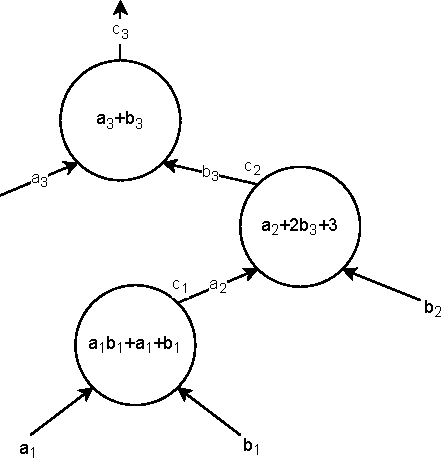
\includegraphics[width=0.4\textwidth]{../figures/plonk-circuit.drawio}
    \caption{Example of a \plonk-like circuit.}
    \label{figure:plonk-circuit-example}
\end{figure}

Observe all the values below depend only on the shape of the circuit itself, so if the circuit does not change, this polynomial should not be recomputed. Check that the \SA, \SB and \SC polynomials are constructed so that we can verify the copy-constraints $c_2 = b_3$ and $c_1 = a_2$ present in the circuit. Observe that equally painted cells have their values swapped, as explained before in the construction of the connection $S$ polynomials.  

\begin{figure}[H]
    \centering
    \begin{tabular}{|c|c|c|c|c|c|c|c|}
        \hline
        \QL	&\QR	&\QM	&\QO	&\QC	&\SA					&\SB						&\SC 							\\ \hline
        1			&1				&1				&-1				&0				&1								&$k_1$								&\cellcolor{pink} $g$				\\
        1			&2				&0				&-1				&3				&\cellcolor{pink}$k_2$			&$k_1 \cdot g$					&\cellcolor{cyan} $k_1 \cdot g^2$	\\
        1			&1				&0				&-1				&0				&$g^2$						&\cellcolor{cyan}$k_2 \cdot g$ &$k_2 \cdot g^2$					\\
        \hline
    \end{tabular}
    \label{table:plonk-circuit-example}
\end{figure}

Therefore, we can derive a PIL program that validates the previous circuit as shown below:
\begin{pil}
    include "config.pil";
    
    namespace Plonk(%N);
    pol constant QL, QR, QM, QO, QC;
    pol constant SA, SB, SC;
    pol constant L1;
    
    pol commit a, b, c;
    
    public pi = a(0);
    
    // Public values check 
    L1 * (a - :pi) = 0;
    
    // Plonk equation 
    pol ab = a*b;
    QL*a + QR*b + QM*ab + QO*c + QC = 0;
    
    // Copy-constraints check 
    {a, b, c} connect {SA, SB, SC};
\end{pil}




%%%%%%%%%%%%%%%%%%%%%%%%%%%%%%%%%%%%%%%%%%%%%%%%%%%%%%%%%%%%%%%%
\subsection{Filling Polynomials}

Until now we have only shown how to specify some kinds of constraints that several polynomials of a certain program described in PIL should satisfy to become \textit{correct}. All these constraints, together with the constant polynomials inherent to the computation itself, specify the transition function underlying the program definition. In other words, changing either any of the constraints or the description of the constant polynomials produces a change in the program we are working on. 

%TODO Check this paragraph
In this section, we are going to use Javascript and \pilcom to generate a specific execution trace for a given PIL. To do so, we are going to compute a valid execution trace for the example of Section \ref{sec:connecting-sm}. As a remark, we will also use the library \texttt{pil-stark} whose utility is to provide a framework to setup, generate and verify proofs, to use a \texttt{FGL} class which mimics a finite field and it is required by some functions that provide the \pilcom package. 

First of all, under the scope of an asynchronous function called \texttt{execute}, we parse the provided PIL (which is, in our case, \texttt{main.pil}) into a Javascript object using the \texttt{compile} function of \pilcom. In code we obtain:
\begin{js}
    const { FGL } = require("pil-stark");
    const { compile } = require("pilcom");
    const path = require("path");
    
    async function execute() {
        const pil = await compile(FGL, path.join(__dirname, "main.pil"));
    }
\end{js}

The \pilcom package also provides two functions that use the \texttt{pil} object to create two crucial objects from it for the construction of the execution trace: the constant polynomials object and the committed polynomials object (using \texttt{newConstPolsArray} and \texttt{newCommitPolsArray} functions, respectively).
\begin{js}
    const { newConstantPolsArray, newCommitPolsArray, compile } = require("pilcom");
    
    async function execute() {
        
        // ... Previous Code
        
        const constPols =  newConstantPolsArray(pil);
        const cmPols = newCommitPolsArray(pil);
    }
\end{js}

Both such objects contain useful information about the PIL itself, such as the provided length of the program $N$, the total number of constant polynomials and the total number of committed polynomials. However, accessing these objects will allow us to fill the entire execution trace for that PIL. We can access a specific position of the execution trace using the syntax:
\begin{js}
    pols.Namespace.Polynomial[i] 
\end{js}
being \texttt{pols} one of the previously introduced \texttt{constPols} and \texttt{cmPols} objects, \texttt{Namespace} being a specific namespace among the ones defined by the PIL files, \texttt{Polynomial} one of the polynomials defined under the scope of the previous namespace and $i$ an integer in the set $[0,N-1]$ representing the row of the current polynomial. Using this we can now start to fill our polynomials. 

In our example, we will use, as inputs for the trace, which are the ones introduced in the \texttt{Main.a} polynomial, an ascending chain of integers from $0$ to $15$ cyclically (because recall that we are only allowed to use $4$ bits integers). We propose here two functions that fill the constant and committed polynomials accordingly. 
\begin{figure}[H]
    \begin{js}
        async function buildConstantPolynomials(constPols, polDeg) {
            
            for (let i=0; i < polDeg; i++) {
                constPols.Global.BITS4[i] = BigInt(i & 0b1111);
                constPols.Global.L1[i] = i === 0 ? 1n : 0n;
                constPols.Negation.RESET[i] = (i % 4) == 3 ? 1n : 0n;
                constPols.Negation.FACTOR[i] = BigInt(1 << (i % 4));
                constPols.Negation.ISLAST[i] = i === polDeg-1 ? 1n : 0n;
            }
        }
    \end{js}
    \caption{Generation of the constant polynomials.}
\end{figure}

\begin{figure}[H]
    \begin{js}
        async function buildcommittedPolynomials(cmPols, polDeg) {
            
            cmPols.Negation.a[-1] = 0n;
            cmPols.Negation.neg_a[-1] = 1n;
            
            for (let i=0; i < polDeg; i++) {
                
                let fourBitsInt = i % 16;
                
                cmPols.Main.a[i] = BigInt(fourBitsInt);
                cmPols.Main.neg_a[i] = BigInt(fourBitsInt ^ 0b1111);
                cmPols.Main.op[i] = FGL.mul(cmPols.Main.a[i], cmPols.Main.neg_a[i]);
                
                cmPols.Multiplier.freeIn1[i] = cmPols.Main.a[i];
                cmPols.Multiplier.freeIn2[i] = cmPols.Main.neg_a[i];
                cmPols.Multiplier.out[i] = cmPols.Main.op[i];
                
                let associatedInt = Math.floor(i/4);
                let bit = (associatedInt >> (i%4) & 1) % 16;
                cmPols.Negation.bits[i] = BigInt(bit);
                cmPols.Negation.nbits[i] = BigInt(bit ^ 1);
                
                
                let factor = BigInt(1 << (i % 4));
                let reset = (i % 4) == 0 ? 1n : 0n;
                cmPols.Negation.a[i] = factor*cmPols.Negation.bits[i] 
                + (1n-reset)*cmPols.Negation.a[i-1];
                cmPols.Negation.neg_a[i] = factor*cmPols.Negation.nbits[i] 
                + (1n-reset)*cmPols.Negation.neg_a[i-1];
            }
        }
    \end{js}
    \caption{Generation of the committed polynomials.}
\end{figure}

Now that we have all the constant and committed polynomials filled in, we can check using a function called \texttt{verifyPil} that they indeed satisfy the constraints defined in the PIL file. We provide below the piece of code that construct the polynomials and check the constraints. If the verification procedure fails, we should not proceed to the proof generation because it will lead to false proof. 
\begin{js}
    const { newConstantPolsArray, newCommitPolsArray, compile, verifyPil } = require("pilcom");
    
    async function execute() {
        
        // ... Previous Code	
        
        const N = constPols.Global.BITS4.length;
        
        await buildConstantPolynomials(constPols, N);
        await buildcommittedPolynomials(cmPols, N);
        
        const res =  await verifyPil(FGL, pil, cmPols , constPols);
        if (res.length != 0) {
            console.log("The execution trace do not satisfy PIL restrictions. Aborting...");
            for (let i=0; i<res.length; i++) {
                console.log(res[i]);
                return;
            }
        }
    }
\end{js}







%TODO: Is this section necessary?
%%%%%%%%%%%%%%%%%%%%%%%%%%%%%%%%%%%%%%%%%%%%%%%%%%%%%%%%%%%%%%%%%
\subsection{Generating a Proof Using \texttt{pil-stark}}

Once the constant and the committed polynomials are filled, we can step to the proof generation stage. We can use the \texttt{pil-stark} Javascript package specially designed to work together with \pilcom to generate STARK proofs about PIL statements. We will use three functions \texttt{starkSetup}, \texttt{starkGen} and \texttt{starkVerify} from the package. The first one is aiming for setting up the STARK, which is independent of the values of committed polynomials. This includes the computation of the tree of the evaluations of the constant polynomials. For executing the setup generation we ought to have an object called \texttt{starkStruct} which is specifying several FRI-related parameters such as the size of the trace domain (which must coincide with $N$, defined in PIL), the size of the extended domain (which together with the previous parameter specifies the correspondent \textit{blowup factor}), the number of queries to be executed and the reduction factors for each of the FRI steps. We execute the setup using the code below:

\begin{js}
    const { FGL, starkSetup } = require("pil-stark");
    
    async function execute() {
        
        // ... Previous Code	
        
        const starkStruct = {
            "nBits": 10,
            "nBitsExt": 11,
            "nQueries": 128,
            "verificationHashType": "GL",
            "steps": [
            {"nBits": 11},
            {"nBits": 5},
            {"nBits": 3},
            {"nBits": 1}
            ]
        };
        
        const setup = await starkSetup(constPols, pil, starkStruct);
    }
\end{js}

Now that we have set up the STARK, we can generate the proof using the \texttt{starkGen} function. We can do this task using the code below. Observe that the \texttt{setup} object contains inside a \texttt{starkInfo} field which contains, aside from all the \texttt{starkStruct} parameters, lots of useful information about the shape of the PIL itself. 

\begin{js}
    const { FGL, starkSetup, starkGen } = require("pil-stark");
    
    async function execute() {
        
        // ... Previous Code	
        
        const resProof = await starkGen(cmPols, constPols, setup.constTree, setup.starkInfo);
    }
\end{js}

Now that a proof has been generated we can be involved in the verification procedure invoking the \texttt{starkVerify} function. This function needs, as arguments, some information provided by the outputs of both the \texttt{starkSetup} and \texttt{starkGen} functions. If the output of the \texttt{starkVerify} function is \texttt{true}, the proof is valid. Otherwise, the verifier should invalidate the proof sent by the prover. 

\begin{js}
    const { FGL, starkSetup, starkGen, starkVerify } = require("pil-stark");
    
    async function execute() {
        
        // ... Previous Code
        
        const resVerify = await starkVerify(
        resP.proof, resP.publics, setup.constRoot, setup.starkInfo
        );
        
        if (resVerify === true) {
            console.log("The proof is VALID!");
        } else {
            console.log("INVALID proof!");
        }
    }
\end{js}


\newpage
\bibliographystyle{alpha}
\bibliography{../cryptobib/abbrev3, ../cryptobib/crypto, ../bib/bibliography}

\end{document}